\documentclass[journal]{IEEEtran}
\usepackage[utf8]{inputenc}
\usepackage{amsmath,amssymb}
\usepackage{booktabs}
\usepackage{graphicx}
\graphicspath{{figures/}}
\usepackage[hyphens]{url}
\usepackage[hidelinks]{hyperref}
\renewcommand{\ttdefault}{cmtt}
% generated by experiments/make_numbers.py from experiments/raw; do not edit
\newcommand{\GeoPerCell}{400}
\newcommand{\GeoCells}{27}
\newcommand{\GeoTotal}{10800}
\newcommand{\GeoNotOut}{9832}
\newcommand{\GeoOut}{614}
\newcommand{\GeoUmp}{354}
\newcommand{\GeoFalseOut}{10}
\newcommand{\GeoMissedOut}{5}
\newcommand{\GeoFalseOutPct}{0.10}
\newcommand{\GeoOutCalledOut}{319}
\newcommand{\GeoAlwaysNotOutPct}{91.0}
\newcommand{\GeoFalseOutParabola}{154}
\newcommand{\GeoAgreeAll}{92.8}
\newcommand{\GeoAgreeAllParabola}{32.3}
\newcommand{\GeoAgreeAllLo}{92.3}
\newcommand{\GeoAgreeAllHi}{93.3}
\newcommand{\GeoFalseOutUpper}{0.17}
\newcommand{\GeoNoVerdict}{34}
\newcommand{\GeoNoVerdictParabola}{1796}
\newcommand{\GeoMedYAll}{2.5}
\newcommand{\GeoMedZAll}{3.6}
\newcommand{\GeoMedYAllParabola}{31.4}
\newcommand{\GeoMedZAllParabola}{39.3}
\newcommand{\GeoMedSpeedErr}{14.2}
\newcommand{\GeoMedContactX}{7.9}
\newcommand{\GeoMedContactY}{1.1}
\newcommand{\GeoAgreeAllUnanch}{71.7}
\newcommand{\GeoFalseOutUnanch}{74}
\newcommand{\GeoMissedOutUnanch}{25}
\newcommand{\GeoOutCalledOutUnanch}{166}
\newcommand{\GeoNoVerdictUnanch}{337}
\newcommand{\GeoUmpCallsAll}{976}
\newcommand{\GeoUmpCallsUnanch}{2899}
\newcommand{\GeoMedYAllUnanch}{4.3}
\newcommand{\GeoMedZAllUnanch}{6.1}
\newcommand{\GeoUnanchFallback}{4176}
\newcommand{\GeoShortLength}{4}
\newcommand{\GeoUnanchFallbackShortPct}{100}
\newcommand{\GeoUnanchFallbackLongPct}{10}
\newcommand{\GeoAnchFallbackShortPct}{1}
\newcommand{\GeoPairN}{6624}
\newcommand{\GeoPairMedYA}{2.1}
\newcommand{\GeoPairMedZA}{3.2}
\newcommand{\GeoPairMedYU}{2.3}
\newcommand{\GeoPairMedZU}{3.8}
\newcommand{\GeoPairPNineZeroYA}{8.1}
\newcommand{\GeoPairPNineZeroYU}{9.8}
\newcommand{\GeoPairPNineZeroZA}{10.1}
\newcommand{\GeoPairPNineZeroZU}{15.9}
\newcommand{\GeoPairAgreeA}{96.0}
\newcommand{\GeoPairAgreeU}{90.9}
\newcommand{\RefAgree}{94.5}
\newcommand{\RefMedY}{2.0}
\newcommand{\RefMedZ}{3.1}
\newcommand{\RefPNineZeroY}{8.3}
\newcommand{\RefPNineZeroZ}{9.1}
\newcommand{\RefAgreeLo}{91.8}
\newcommand{\RefAgreeHi}{96.5}
\newcommand{\GeoFalseOutDistinct}{8}
\newcommand{\GeoFalseOutBowler}{7}
\newcommand{\RefAgreeUnanch}{74.8}
\newcommand{\RefMedYUnanch}{3.4}
\newcommand{\RefMedZUnanch}{4.6}
\newcommand{\RefAgreeParabola}{30.8}
\newcommand{\RefMedYParabola}{28.0}
\newcommand{\RefMedZParabola}{38.1}
\newcommand{\NoiseZeroAgree}{95.8}
\newcommand{\NoiseZeroMedY}{1.9}
\newcommand{\NoiseZeroMedZ}{2.7}
\newcommand{\NoiseZeroUmp}{25}
\newcommand{\NoiseTwoAgree}{92.0}
\newcommand{\NoiseTwoMedY}{2.7}
\newcommand{\NoiseTwoMedZ}{4.4}
\newcommand{\NoiseTwoUmp}{42}
\newcommand{\NoiseThreeAgree}{90.5}
\newcommand{\NoiseThreeMedY}{3.2}
\newcommand{\NoiseThreeMedZ}{5.4}
\newcommand{\NoiseThreeUmp}{48}
\newcommand{\NoiseFiveAgree}{82.0}
\newcommand{\NoiseFiveMedY}{4.8}
\newcommand{\NoiseFiveMedZ}{8.2}
\newcommand{\NoiseFiveUmp}{84}
\newcommand{\FpsThirtyAgree}{93.8}
\newcommand{\FpsThirtyMedY}{2.4}
\newcommand{\FpsThirtyMedZ}{3.5}
\newcommand{\FpsThirtyUmp}{35}
\newcommand{\FpsTwoFortyAgree}{95.0}
\newcommand{\FpsTwoFortyMedY}{2.4}
\newcommand{\FpsTwoFortyMedZ}{3.3}
\newcommand{\FpsTwoFortyUmp}{26}
\newcommand{\TapTwelveAgree}{94.0}
\newcommand{\TapTwelveMedY}{2.7}
\newcommand{\TapTwelveMedZ}{4.2}
\newcommand{\TapTwelveUmp}{27}
\newcommand{\TapEightAgree}{94.0}
\newcommand{\TapEightMedY}{2.2}
\newcommand{\TapEightMedZ}{3.6}
\newcommand{\TapEightUmp}{29}
\newcommand{\DropFortyAgree}{93.2}
\newcommand{\DropFortyMedY}{2.7}
\newcommand{\DropFortyMedZ}{3.8}
\newcommand{\DropFortyUmp}{35}
\newcommand{\PhysOffAgree}{94.5}
\newcommand{\PhysOffMedY}{1.1}
\newcommand{\PhysOffMedZ}{2.4}
\newcommand{\PhysOffUmp}{35}
\newcommand{\PhysOnAgree}{94.5}
\newcommand{\PhysOnMedY}{2.0}
\newcommand{\PhysOnMedZ}{3.1}
\newcommand{\PhysOnUmp}{32}
\newcommand{\SweepAgreeMin}{82.0}
\newcommand{\SweepAgreeMax}{95.8}
\newcommand{\SweepAgreeMinParabola}{25.8}
\newcommand{\SweepAgreeMaxParabola}{37.8}
\newcommand{\SweepAgreeMinUnanch}{57.2}
\newcommand{\SweepAgreeMaxUnanch}{77.5}
\newcommand{\SweepFalseOutMax}{1}
\newcommand{\SweepFalseOutParabolaMax}{10}
\newcommand{\CamStrikerLowAgree}{94.5}
\newcommand{\CamStrikerLowMedY}{2.7}
\newcommand{\CamStrikerLowMedZ}{2.1}
\newcommand{\CamStrikerLowNoVerdict}{2}
\newcommand{\CamStrikerRefAgree}{94.5}
\newcommand{\CamStrikerRefMedY}{2.0}
\newcommand{\CamStrikerRefMedZ}{3.1}
\newcommand{\CamStrikerRefNoVerdict}{1}
\newcommand{\CamStrikerHighAgree}{94.0}
\newcommand{\CamStrikerHighMedY}{2.1}
\newcommand{\CamStrikerHighMedZ}{5.0}
\newcommand{\CamStrikerHighNoVerdict}{0}
\newcommand{\CamStrikerSideAgree}{91.5}
\newcommand{\CamStrikerSideMedY}{4.5}
\newcommand{\CamStrikerSideMedZ}{3.2}
\newcommand{\CamStrikerSideNoVerdict}{0}
\newcommand{\CamBowlerRefAgree}{85.2}
\newcommand{\CamBowlerRefMedY}{4.2}
\newcommand{\CamBowlerRefMedZ}{10.0}
\newcommand{\CamBowlerRefNoVerdict}{10}
\newcommand{\CamBowlerSideAgree}{84.8}
\newcommand{\CamBowlerSideMedY}{7.4}
\newcommand{\CamBowlerSideMedZ}{9.3}
\newcommand{\CamBowlerSideNoVerdict}{2}
\newcommand{\CamStrikerMinAgree}{94.0}
\newcommand{\CamStrikerMaxAgree}{94.5}
\newcommand{\CovYOne}{53.1}
\newcommand{\CovYTwo}{81.5}
\newcommand{\CovYThree}{92.6}
\newcommand{\CovYMedian}{0.92}
\newcommand{\KEmpExpOneYSixtyeight}{1.42}
\newcommand{\KEmpExpOneYNinetyfive}{3.55}
\newcommand{\CovZOne}{63.6}
\newcommand{\CovZTwo}{86.5}
\newcommand{\CovZThree}{93.3}
\newcommand{\CovZMedian}{0.70}
\newcommand{\KEmpExpOneZSixtyeight}{1.14}
\newcommand{\KEmpExpOneZNinetyfive}{3.63}
\newcommand{\BounceObservedPct}{99.7}
\newcommand{\MedSigmaY}{2.6}
\newcommand{\MedSigmaZ}{5.2}
\newcommand{\KZeroAgree}{95.4}
\newcommand{\KZeroFalseOut}{55}
\newcommand{\KZeroUmp}{3.1}
\newcommand{\KZeroMissedOut}{65}
\newcommand{\KZeroUmpInverse}{32}
\newcommand{\KHalfAgree}{93.9}
\newcommand{\KHalfFalseOut}{14}
\newcommand{\KHalfUmp}{6.5}
\newcommand{\KHalfMissedOut}{11}
\newcommand{\KHalfUmpInverse}{15}
\newcommand{\KOneAgree}{92.8}
\newcommand{\KOneFalseOut}{10}
\newcommand{\KOneUmp}{9.0}
\newcommand{\KOneMissedOut}{5}
\newcommand{\KOneUmpInverse}{11}
\newcommand{\KOneHalfAgree}{91.4}
\newcommand{\KOneHalfFalseOut}{4}
\newcommand{\KOneHalfUmp}{10.9}
\newcommand{\KOneHalfMissedOut}{3}
\newcommand{\KOneHalfUmpInverse}{9}
\newcommand{\KTwoAgree}{90.2}
\newcommand{\KTwoFalseOut}{3}
\newcommand{\KTwoUmp}{12.5}
\newcommand{\KTwoMissedOut}{3}
\newcommand{\KTwoUmpInverse}{8}
\newcommand{\EteFalseOutUpper}{3.5}
\newcommand{\EteN}{100}
\newcommand{\EteAgree}{96}
\newcommand{\EteAgreePct}{96.0}
\newcommand{\EteFalseOut}{0}
\newcommand{\EteMissedOut}{0}
\newcommand{\EteUmp}{5}
\newcommand{\EteNoVerdict}{0}
\newcommand{\EteOutTruth}{15}
\newcommand{\EteNotOutTruth}{84}
\newcommand{\EteOutToUmp}{4}
\newcommand{\EteNotOutToUmp}{0}
\newcommand{\EteMedY}{0.9}
\newcommand{\EteMedZ}{1.9}
\newcommand{\EtePNineZeroY}{2.3}
\newcommand{\EtePNineZeroZ}{4.6}
\newcommand{\EteMedContactX}{9.0}
\newcommand{\EteMedContactY}{0.5}
\newcommand{\EteMedSpeedErr}{3.1}
\newcommand{\EteMedReproj}{2.3}
\newcommand{\EteMedTrack}{25}
\newcommand{\EteTapPx}{2}
\newcommand{\EteMedSigmaY}{0.9}
\newcommand{\EteMedSigmaZ}{1.8}
\newcommand{\EteLenTwoAgree}{84}
\newcommand{\EteLenTwoUmp}{4}
\newcommand{\EteLenTwoMedZ}{1.6}
\newcommand{\EteLenFourAgree}{100}
\newcommand{\EteLenFourUmp}{0}
\newcommand{\EteLenFourMedZ}{3.3}
\newcommand{\EteLenSixAgree}{100}
\newcommand{\EteLenSixUmp}{0}
\newcommand{\EteLenSixMedZ}{1.2}
\newcommand{\EteLenEightAgree}{100}
\newcommand{\EteLenEightUmp}{1}
\newcommand{\EteLenEightMedZ}{1.6}
\newcommand{\EteMiddleAgree}{80}
\newcommand{\EteMiddleOutToUmp}{4}
\newcommand{\EteMiddleOutTruth}{15}
\newcommand{\RealTestThreeReproj}{6.3}
\newcommand{\RealTestThreeTrack}{28}
\newcommand{\RealTestThreeLength}{20.1}
\newcommand{\RealTestThreeContactX}{--}
\newcommand{\RealTestThreeResidual}{--}
\newcommand{\RealTestThreeSigmaY}{77.0}
\newcommand{\RealTestThreeSigmaZ}{35.1}
\newcommand{\RealTestThreeSpreadY}{62.6}
\newcommand{\RealTestThreeSpreadZ}{24.9}
\newcommand{\RealTestThreeSpeed}{75}
\newcommand{\RealTestFourReproj}{3.0}
\newcommand{\RealTestFourTrack}{34}
\newcommand{\RealTestFourLength}{4.6}
\newcommand{\RealTestFourContactX}{1.4}
\newcommand{\RealTestFourResidual}{--}
\newcommand{\RealTestFourSigmaY}{3.3}
\newcommand{\RealTestFourSigmaZ}{32.4}
\newcommand{\RealTestFourSpreadY}{12.1}
\newcommand{\RealTestFourSpreadZ}{29.1}
\newcommand{\RealTestFourSpeed}{16}
\newcommand{\RealTestFourPitchMin}{26}
\newcommand{\RealTestFourPitchMax}{28}
\newcommand{\RealTestFourFullSigmaY}{3.3}
\newcommand{\RealTestFourFullSigmaZ}{32.4}
\newcommand{\RealTestFourCalUY}{3.6}
\newcommand{\RealTestFourCalUNinetyfiveY}{8.3}
\newcommand{\RealTestFourCalUZ}{19.9}
\newcommand{\RealTestFourCalUNinetyfiveZ}{48.0}
\newcommand{\RealTestFiveReproj}{6.3}
\newcommand{\RealTestFiveTrack}{29}
\newcommand{\RealTestFiveLength}{2.5}
\newcommand{\RealTestFiveContactX}{1.4}
\newcommand{\RealTestFiveResidual}{--}
\newcommand{\RealTestFiveSigmaY}{5.8}
\newcommand{\RealTestFiveSigmaZ}{2.1}
\newcommand{\RealTestFiveSpreadY}{8.0}
\newcommand{\RealTestFiveSpreadZ}{8.5}
\newcommand{\RealTestFiveSpeed}{24}
\newcommand{\RealTestFivePitchMin}{54}
\newcommand{\RealTestFivePitchMax}{57}
\newcommand{\RealTestFiveFullSigmaY}{5.8}
\newcommand{\RealTestFiveFullSigmaZ}{2.4}
\newcommand{\RealTestFiveCalUY}{6.4}
\newcommand{\RealTestFiveCalUNinetyfiveY}{14.6}
\newcommand{\RealTestFiveCalUZ}{1.6}
\newcommand{\RealTestFiveCalUNinetyfiveZ}{3.9}
\newcommand{\AblAppFocalErr}{1.62}
\newcommand{\AblAppContactX}{6.9}
\newcommand{\AblAppMedY}{2.3}
\newcommand{\AblAppMedZ}{3.2}
\newcommand{\AblAppAgree}{93.5}
\newcommand{\AblAppFalseOut}{1}
\newcommand{\AblPinnedFocalErr}{0.00}
\newcommand{\AblPinnedContactX}{3.9}
\newcommand{\AblPinnedMedY}{2.2}
\newcommand{\AblPinnedMedZ}{3.3}
\newcommand{\AblPinnedAgree}{93.5}
\newcommand{\AblPinnedFalseOut}{1}
\newcommand{\AblFreeLengthFocalErr}{8.39}
\newcommand{\AblFreeLengthContactX}{43.7}
\newcommand{\AblFreeLengthMedY}{2.2}
\newcommand{\AblFreeLengthMedZ}{3.1}
\newcommand{\AblFreeLengthAgree}{93.8}
\newcommand{\AblFreeLengthFalseOut}{1}
\newcommand{\AblWideAppFocalErr}{1.07}
\newcommand{\AblWideAppContactX}{4.5}
\newcommand{\AblWideAppMedY}{2.2}
\newcommand{\AblWideAppMedZ}{3.2}
\newcommand{\AblWideAppAgree}{94.8}
\newcommand{\AblWideAppFalseOut}{0}
\newcommand{\AblWidePinnedFocalErr}{0.00}
\newcommand{\AblWidePinnedContactX}{2.6}
\newcommand{\AblWidePinnedMedY}{2.2}
\newcommand{\AblWidePinnedMedZ}{3.2}
\newcommand{\AblWidePinnedAgree}{94.5}
\newcommand{\AblWidePinnedFalseOut}{0}
\newcommand{\BudRepUcY}{42.8}
\newcommand{\BudRepUcNoSamplerY}{39.4}
\newcommand{\BudRepPipeSigmaY}{9.4}
\newcommand{\BudDistUcMedY}{46.9}
\newcommand{\BudDistUcPNinetyY}{88.3}
\newcommand{\BudDistUcMedWithSamplerY}{64.3}
\newcommand{\BudDistDominantY}{swing Cs}
\newcommand{\BudDistDominantCountY}{68}
\newcommand{\BudRepTopY}{swing Cs}
\newcommand{\BudRepTopYMm}{38.2}
\newcommand{\BudRepSecondY}{ball centre}
\newcommand{\BudRepSecondYMm}{7.3}
\newcommand{\BudRepUcZ}{108.3}
\newcommand{\BudRepUcNoSamplerZ}{65.3}
\newcommand{\BudRepPipeSigmaZ}{44.6}
\newcommand{\BudDistUcMedZ}{53.8}
\newcommand{\BudDistUcPNinetyZ}{143.7}
\newcommand{\BudDistUcMedWithSamplerZ}{86.4}
\newcommand{\BudDistDominantZ}{swing Cs}
\newcommand{\BudDistDominantCountZ}{35}
\newcommand{\BudRepTopZ}{swing Cs}
\newcommand{\BudRepTopZMm}{46.5}
\newcommand{\BudRepSecondZ}{ball centre}
\newcommand{\BudRepSecondZMm}{35.2}
\newcommand{\BudDistN}{100}
\newcommand{\BudSamplerY}{16.7}
\newcommand{\BudSamplerZ}{86.4}
\newcommand{\McM}{30000}
\newcommand{\McBatches}{3}
\newcommand{\McStable}{no}
\newcommand{\McFailed}{0}
\newcommand{\McUcY}{39.4}
\newcommand{\McUY}{55.0}
\newcommand{\McMeanY}{-7.4}
\newcommand{\McLowY}{-129.5}
\newcommand{\McHighY}{104.8}
\newcommand{\McGumY}{1.5}
\newcommand{\McGumLowY}{-75.7}
\newcommand{\McGumHighY}{78.7}
\newcommand{\McDLowY}{53.8}
\newcommand{\McDHighY}{26.1}
\newcommand{\McDeltaY}{0.5}
\newcommand{\McValidY}{fails}
\newcommand{\McRatioY}{1.40}
\newcommand{\McUcZ}{65.3}
\newcommand{\McUZ}{53.6}
\newcommand{\McMeanZ}{-47.7}
\newcommand{\McLowZ}{-158.8}
\newcommand{\McHighZ}{52.3}
\newcommand{\McGumZ}{8.7}
\newcommand{\McGumLowZ}{-119.4}
\newcommand{\McGumHighZ}{136.8}
\newcommand{\McDLowZ}{39.5}
\newcommand{\McDHighZ}{84.5}
\newcommand{\McDeltaZ}{0.5}
\newcommand{\McValidZ}{fails}
\newcommand{\McRatioZ}{0.82}
\newcommand{\McSubN}{10}
\newcommand{\McSubTrials}{1000}
\newcommand{\McSubValidY}{0}
\newcommand{\McSubValidZ}{0}
\newcommand{\McSubRatioMinY}{0.34}
\newcommand{\McSubRatioMaxY}{1.80}
\newcommand{\McSubRatioMedY}{1.11}
\newcommand{\McSubRatioMinZ}{0.22}
\newcommand{\McSubRatioMaxZ}{1.46}
\newcommand{\McSubRatioMedZ}{0.87}
\newcommand{\McTwoSMaxY}{2.8}
\newcommand{\McPipeSigmaMedY}{27.2}
\newcommand{\McTwoSMaxZ}{2.4}
\newcommand{\McPipeSigmaMedZ}{53.7}
\newcommand{\BudGrpTapsRepY}{3.0}
\newcommand{\BudGrpTapsMedY}{3.4}
\newcommand{\BudGrpTapsRepZ}{4.8}
\newcommand{\BudGrpTapsMedZ}{4.8}
\newcommand{\BudGrpBallRepY}{7.3}
\newcommand{\BudGrpBallMedY}{15.6}
\newcommand{\BudGrpBallRepZ}{35.2}
\newcommand{\BudGrpBallMedZ}{25.1}
\newcommand{\BudGrpTimingRepY}{3.0}
\newcommand{\BudGrpTimingMedY}{9.5}
\newcommand{\BudGrpTimingRepZ}{16.5}
\newcommand{\BudGrpTimingMedZ}{14.9}
\newcommand{\BudGrpSceneRepY}{1.4}
\newcommand{\BudGrpSceneMedY}{4.1}
\newcommand{\BudGrpSceneRepZ}{12.6}
\newcommand{\BudGrpSceneMedZ}{15.3}
\newcommand{\BudGrpLensRepY}{0.1}
\newcommand{\BudGrpLensMedY}{0.2}
\newcommand{\BudGrpLensRepZ}{0.7}
\newcommand{\BudGrpLensMedZ}{0.9}
\newcommand{\BudGrpFlightRepY}{38.5}
\newcommand{\BudGrpFlightMedY}{37.9}
\newcommand{\BudGrpFlightRepZ}{50.8}
\newcommand{\BudGrpFlightMedZ}{37.7}
\newcommand{\BudRepMeasY}{8.5}
\newcommand{\BudRepMeasZ}{41.1}
\newcommand{\CovBN}{600}
\newcommand{\CovBFitted}{599}
\newcommand{\CovBBounce}{599}
\newcommand{\CovBFitPitchOne}{23.7}
\newcommand{\CovBFitPitchNinetyfive}{48.9}
\newcommand{\CovBFitPitchRatio}{2.03}
\newcommand{\CovBFitCreaseOne}{44.2}
\newcommand{\CovBFitCreaseNinetyfive}{71.1}
\newcommand{\CovBFitCreaseRatio}{1.20}
\newcommand{\CovBFitYOne}{53.6}
\newcommand{\CovBFitYNinetyfive}{84.1}
\newcommand{\CovBFitYRatio}{0.93}
\newcommand{\CovBFitZOne}{60.8}
\newcommand{\CovBFitZNinetyfive}{85.3}
\newcommand{\CovBFitZRatio}{0.79}
\newcommand{\CovBFitCalPitchOne}{43.6}
\newcommand{\CovBFitCalPitchNinetyfive}{71.6}
\newcommand{\CovBFitCalPitchRatio}{1.17}
\newcommand{\CovBFitCalCreaseOne}{47.9}
\newcommand{\CovBFitCalCreaseNinetyfive}{74.5}
\newcommand{\CovBFitCalCreaseRatio}{1.06}
\newcommand{\CovBFitCalYOne}{56.4}
\newcommand{\CovBFitCalYNinetyfive}{85.8}
\newcommand{\CovBFitCalYRatio}{0.90}
\newcommand{\CovBFitCalZOne}{61.4}
\newcommand{\CovBFitCalZNinetyfive}{86.3}
\newcommand{\CovBFitCalZRatio}{0.78}
\newcommand{\CovBFullPitchOne}{69.8}
\newcommand{\CovBFullPitchNinetyfive}{92.8}
\newcommand{\CovBFullPitchRatio}{0.64}
\newcommand{\CovBFullCreaseOne}{74.6}
\newcommand{\CovBFullCreaseNinetyfive}{91.2}
\newcommand{\CovBFullCreaseRatio}{0.49}
\newcommand{\CovBFullYOne}{63.9}
\newcommand{\CovBFullYNinetyfive}{90.7}
\newcommand{\CovBFullYRatio}{0.72}
\newcommand{\CovBFullZOne}{85.5}
\newcommand{\CovBFullZNinetyfive}{97.7}
\newcommand{\CovBFullZRatio}{0.43}
\newcommand{\CalPitchCovSixtyeight}{68.3}
\newcommand{\CalPitchCovSixtyeightLo}{64.4}
\newcommand{\CalPitchCovSixtyeightHi}{72.0}
\newcommand{\CalPitchKSixtyeight}{0.98}
\newcommand{\CalPitchKSixtyeightMin}{0.97}
\newcommand{\CalPitchKSixtyeightMax}{0.99}
\newcommand{\CalPitchCovNinetyfive}{95.0}
\newcommand{\CalPitchCovNinetyfiveLo}{92.9}
\newcommand{\CalPitchCovNinetyfiveHi}{96.6}
\newcommand{\CalPitchKNinetyfive}{2.16}
\newcommand{\CalPitchKNinetyfiveMin}{2.10}
\newcommand{\CalPitchKNinetyfiveMax}{2.22}
\newcommand{\CalPitchMedU}{14.1}
\newcommand{\CalPitchMedUNinetyfive}{31.1}
\newcommand{\CalPitchMeanBefore}{-1.7}
\newcommand{\CalPitchMeanAfter}{-1.7}
\newcommand{\CalPitchMeanSe}{1.0}
\newcommand{\CalCreaseCovSixtyeight}{68.8}
\newcommand{\CalCreaseCovSixtyeightLo}{64.9}
\newcommand{\CalCreaseCovSixtyeightHi}{72.5}
\newcommand{\CalCreaseKSixtyeight}{0.83}
\newcommand{\CalCreaseKSixtyeightMin}{0.81}
\newcommand{\CalCreaseKSixtyeightMax}{0.87}
\newcommand{\CalCreaseCovNinetyfive}{95.3}
\newcommand{\CalCreaseCovNinetyfiveLo}{93.3}
\newcommand{\CalCreaseCovNinetyfiveHi}{96.9}
\newcommand{\CalCreaseKNinetyfive}{2.50}
\newcommand{\CalCreaseKNinetyfiveMin}{2.43}
\newcommand{\CalCreaseKNinetyfiveMax}{2.68}
\newcommand{\CalCreaseMedU}{22.9}
\newcommand{\CalCreaseMedUNinetyfive}{69.5}
\newcommand{\CalCreaseMeanBefore}{3.7}
\newcommand{\CalCreaseMeanAfter}{3.7}
\newcommand{\CalCreaseMeanSe}{1.9}
\newcommand{\CalYCovSixtyeight}{68.6}
\newcommand{\CalYCovSixtyeightLo}{64.7}
\newcommand{\CalYCovSixtyeightHi}{72.3}
\newcommand{\CalYKSixtyeight}{1.09}
\newcommand{\CalYKSixtyeightMin}{1.06}
\newcommand{\CalYKSixtyeightMax}{1.12}
\newcommand{\CalYCovNinetyfive}{95.2}
\newcommand{\CalYCovNinetyfiveLo}{93.1}
\newcommand{\CalYCovNinetyfiveHi}{96.7}
\newcommand{\CalYKNinetyfive}{2.51}
\newcommand{\CalYKNinetyfiveMin}{2.44}
\newcommand{\CalYKNinetyfiveMax}{2.55}
\newcommand{\CalYMedU}{30.7}
\newcommand{\CalYMedUNinetyfive}{69.7}
\newcommand{\CalYMeanBefore}{5.6}
\newcommand{\CalYMeanAfter}{5.6}
\newcommand{\CalYMeanSe}{3.0}
\newcommand{\CalYSwingCorr}{0.09}
\newcommand{\CalYSwingRsq}{16}
\newcommand{\CalZCovSixtyeight}{68.4}
\newcommand{\CalZCovSixtyeightLo}{64.6}
\newcommand{\CalZCovSixtyeightHi}{72.2}
\newcommand{\CalZKSixtyeight}{0.61}
\newcommand{\CalZKSixtyeightMin}{0.60}
\newcommand{\CalZKSixtyeightMax}{0.66}
\newcommand{\CalZCovNinetyfive}{95.2}
\newcommand{\CalZCovNinetyfiveLo}{93.1}
\newcommand{\CalZCovNinetyfiveHi}{96.7}
\newcommand{\CalZKNinetyfive}{1.48}
\newcommand{\CalZKNinetyfiveMin}{1.42}
\newcommand{\CalZKNinetyfiveMax}{1.58}
\newcommand{\CalZMedU}{50.7}
\newcommand{\CalZMedUNinetyfive}{120.9}
\newcommand{\CalZMeanBefore}{-18.3}
\newcommand{\CalZMeanAfter}{-0.1}
\newcommand{\CalZMeanSe}{3.8}
\newcommand{\CalZSwingCorr}{-0.01}
\newcommand{\CalZSwingRsq}{1}
\newcommand{\CalBiasA}{-5.3}
\newcommand{\CalBiasUA}{12.1}
\newcommand{\CalBiasC}{-2.17}
\newcommand{\CalBiasUC}{1.92}
\newcommand{\CalBiasMedU}{5.4}
\newcommand{\CalN}{599}
\newcommand{\KEmpFitYSixtyeight}{1.32}
\newcommand{\KEmpFitYNinetyfive}{2.99}
\newcommand{\KEmpFitZSixtyeight}{1.25}
\newcommand{\KEmpFitZNinetyfive}{3.10}
\newcommand{\KEmpFitCalYSixtyeight}{1.28}
\newcommand{\KEmpFitCalYNinetyfive}{2.84}
\newcommand{\KEmpFitCalZSixtyeight}{1.23}
\newcommand{\KEmpFitCalZNinetyfive}{2.91}
\newcommand{\KEmpFullYSixtyeight}{1.09}
\newcommand{\KEmpFullYNinetyfive}{2.47}
\newcommand{\KEmpFullZSixtyeight}{0.66}
\newcommand{\KEmpFullZNinetyfive}{1.53}
\newcommand{\ModPitchForm}{constant}
\newcommand{\ModPitchParamOne}{11.74}
\newcommand{\ModPitchMeanErr}{-1.7}
\newcommand{\ModPitchMedErr}{9.5}
\newcommand{\ModPitchSigFit}{4.7}
\newcommand{\ModPitchSigCal}{6.3}
\newcommand{\ModPitchSigMod}{11.7}
\newcommand{\ModCreaseForm}{constant + proportional}
\newcommand{\ModCreaseParamOne}{16.77}
\newcommand{\ModCreaseParamTwo}{2.31}
\newcommand{\ModCreaseMeanErr}{3.7}
\newcommand{\ModCreaseMedErr}{13.2}
\newcommand{\ModCreaseSigFit}{12.9}
\newcommand{\ModCreaseSigCal}{3.4}
\newcommand{\ModCreaseSigMod}{21.8}
\newcommand{\ModYForm}{proportional to x_b}
\newcommand{\ModYParamOne}{1.95}
\newcommand{\ModYMeanErr}{5.6}
\newcommand{\ModYMedErr}{20.2}
\newcommand{\ModYSigFit}{23.5}
\newcommand{\ModYSigCal}{3.7}
\newcommand{\ModYSigMod}{11.2}
\newcommand{\ModZForm}{proportional to x_b}
\newcommand{\ModZParamOne}{9.33}
\newcommand{\ModZMeanErr}{-18.3}
\newcommand{\ModZMedErr}{36.2}
\newcommand{\ModZSigFit}{46.9}
\newcommand{\ModZSigCal}{5.2}
\newcommand{\ModZSigMod}{54.0}
\newcommand{\SwRsZeroMedY}{17.4}
\newcommand{\SwRsZeroMeanY}{5.2}
\newcommand{\SwRsZeroCovFitY}{55.3}
\newcommand{\SwRsZeroCovFullY}{64.3}
\newcommand{\SwRsZeroMedZ}{35.1}
\newcommand{\SwRsZeroMeanZ}{-11.4}
\newcommand{\SwRsZeroCovFitZ}{58.8}
\newcommand{\SwRsZeroCovFullZ}{85.4}
\newcommand{\SwRsThirtyMedY}{20.2}
\newcommand{\SwRsThirtyMeanY}{-4.2}
\newcommand{\SwRsThirtyCovFitY}{56.8}
\newcommand{\SwRsThirtyCovFullY}{67.8}
\newcommand{\SwRsThirtyMedZ}{31.2}
\newcommand{\SwRsThirtyMeanZ}{-8.7}
\newcommand{\SwRsThirtyCovFitZ}{63.3}
\newcommand{\SwRsThirtyCovFullZ}{85.4}
\newcommand{\SwRsThirtyCorrMedY}{18.6}
\newcommand{\SwRsThirtyCorrMeanY}{4.6}
\newcommand{\SwRsThirtyCorrCovFitY}{57.8}
\newcommand{\SwRsThirtyCorrCovFullY}{69.3}
\newcommand{\SwRsThirtyCorrMedZ}{32.7}
\newcommand{\SwRsThirtyCorrMeanZ}{-10.9}
\newcommand{\SwRsThirtyCorrCovFitZ}{63.8}
\newcommand{\SwRsThirtyCorrCovFullZ}{86.4}
\newcommand{\SwRsMinusThirtyMedY}{20.8}
\newcommand{\SwRsMinusThirtyMeanY}{13.7}
\newcommand{\SwRsMinusThirtyCovFitY}{54.8}
\newcommand{\SwRsMinusThirtyCovFullY}{65.8}
\newcommand{\SwRsMinusThirtyMedZ}{38.0}
\newcommand{\SwRsMinusThirtyMeanZ}{-14.9}
\newcommand{\SwRsMinusThirtyCovFitZ}{61.8}
\newcommand{\SwRsMinusThirtyCovFullZ}{84.9}
\newcommand{\SwSampTsMedY}{18.6}
\newcommand{\SwSampTsMeanY}{4.2}
\newcommand{\SwSampTsCovFitY}{54.3}
\newcommand{\SwSampTsCovFullY}{66.8}
\newcommand{\SwSampTsMedZ}{31.2}
\newcommand{\SwSampTsMeanZ}{-6.6}
\newcommand{\SwSampTsCovFitZ}{62.8}
\newcommand{\SwSampTsCovFullZ}{86.4}
\newcommand{\SwSampTsMetaMedY}{18.9}
\newcommand{\SwSampTsMetaMeanY}{4.4}
\newcommand{\SwSampTsMetaCovFitY}{52.8}
\newcommand{\SwSampTsMetaCovFullY}{67.3}
\newcommand{\SwSampTsMetaMedZ}{32.7}
\newcommand{\SwSampTsMetaMeanZ}{-9.8}
\newcommand{\SwSampTsMetaCovFitZ}{62.3}
\newcommand{\SwSampTsMetaCovFullZ}{84.9}
\newcommand{\SwSampFixedMedY}{18.9}
\newcommand{\SwSampFixedMeanY}{4.0}
\newcommand{\SwSampFixedCovFitY}{53.3}
\newcommand{\SwSampFixedCovFullY}{68.3}
\newcommand{\SwSampFixedMedZ}{36.3}
\newcommand{\SwSampFixedMeanZ}{-9.0}
\newcommand{\SwSampFixedCovFitZ}{59.3}
\newcommand{\SwSampFixedCovFullZ}{82.4}
\newcommand{\SwSampFixedMetaMedY}{19.7}
\newcommand{\SwSampFixedMetaMeanY}{4.5}
\newcommand{\SwSampFixedMetaCovFitY}{52.8}
\newcommand{\SwSampFixedMetaCovFullY}{67.3}
\newcommand{\SwSampFixedMetaMedZ}{34.1}
\newcommand{\SwSampFixedMetaMeanZ}{-11.9}
\newcommand{\SwSampFixedMetaCovFitZ}{61.8}
\newcommand{\SwSampFixedMetaCovFullZ}{83.9}
\newcommand{\SwSampSubmittedMedY}{26.7}
\newcommand{\SwSampSubmittedMeanY}{0.2}
\newcommand{\SwSampSubmittedCovFitY}{52.3}
\newcommand{\SwSampSubmittedCovFullY}{58.3}
\newcommand{\SwSampSubmittedMedZ}{52.0}
\newcommand{\SwSampSubmittedMeanZ}{-22.0}
\newcommand{\SwSampSubmittedCovFitZ}{53.3}
\newcommand{\SwSampSubmittedCovFullZ}{77.9}
\newcommand{\SwSampSubmittedMetaMedY}{25.8}
\newcommand{\SwSampSubmittedMetaMeanY}{5.8}
\newcommand{\SwSampSubmittedMetaCovFitY}{55.3}
\newcommand{\SwSampSubmittedMetaCovFullY}{62.8}
\newcommand{\SwSampSubmittedMetaMedZ}{45.9}
\newcommand{\SwSampSubmittedMetaMeanZ}{-19.8}
\newcommand{\SwSampSubmittedMetaCovFitZ}{57.8}
\newcommand{\SwSampSubmittedMetaCovFullZ}{79.9}
\newcommand{\RiskN}{599}
\newcommand{\RiskTruthOut}{39}
\newcommand{\RiskTruthUmp}{15}
\newcommand{\RiskTruthNotOut}{545}
\newcommand{\RiskBoundSingleOne}{2.33}
\newcommand{\RiskBoundFourOne}{2.81}
\newcommand{\RiskBoundSingleFive}{1.64}
\newcommand{\RiskBoundFourFive}{2.23}
\newcommand{\RiskFitKOne}{2.25}
\newcommand{\RiskFitKGlobalOne}{0.00}
\newcommand{\RiskFitAgreeOne}{92.0}
\newcommand{\RiskFitUmpOne}{10.5}
\newcommand{\RiskFitOutOne}{3.2}
\newcommand{\RiskFitFalseOutOne}{0}
\newcommand{\RiskFitMissedOutOne}{0}
\newcommand{\RiskFitFalseOutCpOne}{0.50}
\newcommand{\RiskFitOutToUmpOne}{51.3}
\newcommand{\RiskFitKFive}{1.20}
\newcommand{\RiskFitKGlobalFive}{0.00}
\newcommand{\RiskFitAgreeFive}{95.0}
\newcommand{\RiskFitUmpFive}{7.0}
\newcommand{\RiskFitOutFive}{5.0}
\newcommand{\RiskFitFalseOutFive}{1}
\newcommand{\RiskFitMissedOutFive}{0}
\newcommand{\RiskFitFalseOutCpFive}{0.79}
\newcommand{\RiskFitOutToUmpFive}{28.2}
\newcommand{\RiskFitKOneAgree}{95.8}
\newcommand{\RiskFitKOneUmp}{6.2}
\newcommand{\RiskFitKOneFalseOut}{1}
\newcommand{\RiskFitKOneMaxSpec}{6.0}
\newcommand{\RiskFitKOneMissedOut}{0}
\newcommand{\RiskFitKZeroAgree}{97.2}
\newcommand{\RiskFitKZeroFalseOut}{3}
\newcommand{\RiskFitKZeroMaxSpec}{92.9}
\newcommand{\RiskFitCalKOne}{1.80}
\newcommand{\RiskFitCalKGlobalOne}{0.00}
\newcommand{\RiskFitCalAgreeOne}{93.0}
\newcommand{\RiskFitCalUmpOne}{9.5}
\newcommand{\RiskFitCalOutOne}{3.7}
\newcommand{\RiskFitCalFalseOutOne}{0}
\newcommand{\RiskFitCalMissedOutOne}{0}
\newcommand{\RiskFitCalFalseOutCpOne}{0.50}
\newcommand{\RiskFitCalOutToUmpOne}{43.6}
\newcommand{\RiskFitCalKFive}{1.45}
\newcommand{\RiskFitCalKGlobalFive}{0.00}
\newcommand{\RiskFitCalAgreeFive}{94.3}
\newcommand{\RiskFitCalUmpFive}{8.2}
\newcommand{\RiskFitCalOutFive}{4.2}
\newcommand{\RiskFitCalFalseOutFive}{0}
\newcommand{\RiskFitCalMissedOutFive}{0}
\newcommand{\RiskFitCalFalseOutCpFive}{0.50}
\newcommand{\RiskFitCalOutToUmpFive}{35.9}
\newcommand{\RiskFitCalKOneAgree}{95.5}
\newcommand{\RiskFitCalKOneUmp}{6.5}
\newcommand{\RiskFitCalKOneFalseOut}{1}
\newcommand{\RiskFitCalKOneMaxSpec}{7.6}
\newcommand{\RiskFitCalKOneMissedOut}{0}
\newcommand{\RiskFitCalKZeroAgree}{97.2}
\newcommand{\RiskFitCalKZeroFalseOut}{3}
\newcommand{\RiskFitCalKZeroMaxSpec}{92.9}
\newcommand{\RiskFullKOne}{1.85}
\newcommand{\RiskFullKGlobalOne}{0.00}
\newcommand{\RiskFullAgreeOne}{89.5}
\newcommand{\RiskFullUmpOne}{13.0}
\newcommand{\RiskFullOutOne}{2.2}
\newcommand{\RiskFullFalseOutOne}{0}
\newcommand{\RiskFullMissedOutOne}{0}
\newcommand{\RiskFullFalseOutCpOne}{0.50}
\newcommand{\RiskFullOutToUmpOne}{66.7}
\newcommand{\RiskFullKFive}{1.00}
\newcommand{\RiskFullKGlobalFive}{0.00}
\newcommand{\RiskFullAgreeFive}{93.8}
\newcommand{\RiskFullUmpFive}{8.3}
\newcommand{\RiskFullOutFive}{4.3}
\newcommand{\RiskFullFalseOutFive}{0}
\newcommand{\RiskFullMissedOutFive}{0}
\newcommand{\RiskFullFalseOutCpFive}{0.50}
\newcommand{\RiskFullOutToUmpFive}{35.9}
\newcommand{\RiskFullKOneAgree}{93.8}
\newcommand{\RiskFullKOneUmp}{8.3}
\newcommand{\RiskFullKOneFalseOut}{0}
\newcommand{\RiskFullKOneMaxSpec}{4.6}
\newcommand{\RiskFullKOneMissedOut}{0}
\newcommand{\RiskFullKZeroAgree}{97.2}
\newcommand{\RiskFullKZeroFalseOut}{3}
\newcommand{\RiskFullKZeroMaxSpec}{92.9}
\newcommand{\RiskCalKOne}{1.75}
\newcommand{\RiskCalKGlobalOne}{0.00}
\newcommand{\RiskCalAgreeOne}{89.0}
\newcommand{\RiskCalUmpOne}{13.5}
\newcommand{\RiskCalOutOne}{2.0}
\newcommand{\RiskCalFalseOutOne}{0}
\newcommand{\RiskCalMissedOutOne}{0}
\newcommand{\RiskCalFalseOutCpOne}{0.50}
\newcommand{\RiskCalOutToUmpOne}{69.2}
\newcommand{\RiskCalKFive}{1.15}
\newcommand{\RiskCalKGlobalFive}{0.00}
\newcommand{\RiskCalAgreeFive}{92.3}
\newcommand{\RiskCalUmpFive}{10.2}
\newcommand{\RiskCalOutFive}{3.3}
\newcommand{\RiskCalFalseOutFive}{0}
\newcommand{\RiskCalMissedOutFive}{0}
\newcommand{\RiskCalFalseOutCpFive}{0.50}
\newcommand{\RiskCalOutToUmpFive}{48.7}
\newcommand{\RiskCalKOneAgree}{93.5}
\newcommand{\RiskCalKOneUmp}{8.7}
\newcommand{\RiskCalKOneFalseOut}{0}
\newcommand{\RiskCalKOneMaxSpec}{7.1}
\newcommand{\RiskCalKOneMissedOut}{0}
\newcommand{\RiskCalKZeroAgree}{97.3}
\newcommand{\RiskCalKZeroFalseOut}{3}
\newcommand{\RiskCalKZeroMaxSpec}{93.0}
\newcommand{\RiskShippedMaxSpecFull}{27.6}
\newcommand{\RiskShippedMeanSpecFull}{2.9}
\newcommand{\RiskShippedOutsOverFive}{4}
\newcommand{\RiskShippedOutToUmp}{17.9}
\newcommand{\RiskShippedMaxSpecCal}{30.3}
\newcommand{\RiskShippedOutsOverFiveCal}{7}
\newcommand{\PhysBaselineMedY}{9.9}
\newcommand{\PhysBaselineMedZ}{20.6}
\newcommand{\PhysBaselineMeanY}{-1.8}
\newcommand{\PhysBaselineMeanZ}{6.0}
\newcommand{\PhysBaselineCovFullY}{82.4}
\newcommand{\PhysBaselineCovFullZ}{96.0}
\newcommand{\PhysBaselineCovFitY}{70.9}
\newcommand{\PhysBaselineCovFitZ}{78.4}
\newcommand{\PhysBaselineAgreeFit}{96.0}
\newcommand{\PhysBaselineUmpFit}{7.5}
\newcommand{\PhysBaselineAgreeFull}{87.4}
\newcommand{\PhysBaselineUmpFull}{16.1}
\newcommand{\PhysBaselineAgreeFullAlt}{93.5}
\newcommand{\PhysBaselineUmpFullAlt}{10.1}
\newcommand{\PhysDragCdZeroThreeFiveMedY}{10.3}
\newcommand{\PhysDragCdZeroThreeFiveMedZ}{22.9}
\newcommand{\PhysDragCdZeroThreeFiveMeanY}{-0.4}
\newcommand{\PhysDragCdZeroThreeFiveMeanZ}{-1.3}
\newcommand{\PhysDragCdZeroThreeFiveCovFullY}{86.5}
\newcommand{\PhysDragCdZeroThreeFiveCovFullZ}{94.0}
\newcommand{\PhysDragCdZeroThreeFiveCovFitY}{70.5}
\newcommand{\PhysDragCdZeroThreeFiveCovFitZ}{76.0}
\newcommand{\PhysDragCdZeroThreeFiveAgreeFit}{96.0}
\newcommand{\PhysDragCdZeroThreeFiveUmpFit}{8.0}
\newcommand{\PhysDragCdZeroThreeFiveAgreeFull}{87.5}
\newcommand{\PhysDragCdZeroThreeFiveUmpFull}{16.5}
\newcommand{\PhysDragCdZeroThreeFiveAgreeFullAlt}{93.0}
\newcommand{\PhysDragCdZeroThreeFiveUmpFullAlt}{11.0}
\newcommand{\PhysDragCdZeroFourFiveMedY}{10.6}
\newcommand{\PhysDragCdZeroFourFiveMedZ}{25.1}
\newcommand{\PhysDragCdZeroFourFiveMeanY}{-0.2}
\newcommand{\PhysDragCdZeroFourFiveMeanZ}{-4.2}
\newcommand{\PhysDragCdZeroFourFiveCovFullY}{80.9}
\newcommand{\PhysDragCdZeroFourFiveCovFullZ}{92.0}
\newcommand{\PhysDragCdZeroFourFiveCovFitY}{69.3}
\newcommand{\PhysDragCdZeroFourFiveCovFitZ}{73.4}
\newcommand{\PhysDragCdZeroFourFiveAgreeFit}{97.0}
\newcommand{\PhysDragCdZeroFourFiveUmpFit}{7.0}
\newcommand{\PhysDragCdZeroFourFiveAgreeFull}{88.9}
\newcommand{\PhysDragCdZeroFourFiveUmpFull}{15.1}
\newcommand{\PhysDragCdZeroFourFiveAgreeFullAlt}{93.0}
\newcommand{\PhysDragCdZeroFourFiveUmpFullAlt}{11.1}
\newcommand{\PhysDragCdZeroFiveFiveMedY}{12.0}
\newcommand{\PhysDragCdZeroFiveFiveMedZ}{27.9}
\newcommand{\PhysDragCdZeroFiveFiveMeanY}{-1.0}
\newcommand{\PhysDragCdZeroFiveFiveMeanZ}{-10.2}
\newcommand{\PhysDragCdZeroFiveFiveCovFullY}{79.5}
\newcommand{\PhysDragCdZeroFiveFiveCovFullZ}{90.0}
\newcommand{\PhysDragCdZeroFiveFiveCovFitY}{66.5}
\newcommand{\PhysDragCdZeroFiveFiveCovFitZ}{71.5}
\newcommand{\PhysDragCdZeroFiveFiveAgreeFit}{98.0}
\newcommand{\PhysDragCdZeroFiveFiveUmpFit}{6.5}
\newcommand{\PhysDragCdZeroFiveFiveAgreeFull}{89.5}
\newcommand{\PhysDragCdZeroFiveFiveUmpFull}{15.0}
\newcommand{\PhysDragCdZeroFiveFiveAgreeFullAlt}{95.0}
\newcommand{\PhysDragCdZeroFiveFiveUmpFullAlt}{9.5}
\newcommand{\PhysSwingCsZeroOneMedY}{17.3}
\newcommand{\PhysSwingCsZeroOneMedZ}{23.8}
\newcommand{\PhysSwingCsZeroOneMeanY}{1.0}
\newcommand{\PhysSwingCsZeroOneMeanZ}{-5.8}
\newcommand{\PhysSwingCsZeroOneCovFullY}{77.9}
\newcommand{\PhysSwingCsZeroOneCovFullZ}{95.0}
\newcommand{\PhysSwingCsZeroOneCovFitY}{63.3}
\newcommand{\PhysSwingCsZeroOneCovFitZ}{80.9}
\newcommand{\PhysSwingCsZeroOneAgreeFit}{95.5}
\newcommand{\PhysSwingCsZeroOneUmpFit}{5.5}
\newcommand{\PhysSwingCsZeroOneAgreeFull}{86.9}
\newcommand{\PhysSwingCsZeroOneUmpFull}{14.1}
\newcommand{\PhysSwingCsZeroOneAgreeFullAlt}{92.0}
\newcommand{\PhysSwingCsZeroOneUmpFullAlt}{9.0}
\newcommand{\PhysSwingCsZeroTwoMedY}{29.1}
\newcommand{\PhysSwingCsZeroTwoMedZ}{28.6}
\newcommand{\PhysSwingCsZeroTwoMeanY}{1.4}
\newcommand{\PhysSwingCsZeroTwoMeanZ}{-29.2}
\newcommand{\PhysSwingCsZeroTwoCovFullY}{72.5}
\newcommand{\PhysSwingCsZeroTwoCovFullZ}{94.5}
\newcommand{\PhysSwingCsZeroTwoCovFitY}{62.5}
\newcommand{\PhysSwingCsZeroTwoCovFitZ}{79.0}
\newcommand{\PhysSwingCsZeroTwoAgreeFit}{94.5}
\newcommand{\PhysSwingCsZeroTwoUmpFit}{9.0}
\newcommand{\PhysSwingCsZeroTwoAgreeFull}{90.5}
\newcommand{\PhysSwingCsZeroTwoUmpFull}{14.0}
\newcommand{\PhysSwingCsZeroTwoAgreeFullAlt}{94.5}
\newcommand{\PhysSwingCsZeroTwoUmpFullAlt}{10.0}
\newcommand{\PhysSwingCsZeroThreeMedY}{43.8}
\newcommand{\PhysSwingCsZeroThreeMedZ}{36.3}
\newcommand{\PhysSwingCsZeroThreeMeanY}{-1.4}
\newcommand{\PhysSwingCsZeroThreeMeanZ}{-52.1}
\newcommand{\PhysSwingCsZeroThreeCovFullY}{72.5}
\newcommand{\PhysSwingCsZeroThreeCovFullZ}{93.5}
\newcommand{\PhysSwingCsZeroThreeCovFitY}{67.0}
\newcommand{\PhysSwingCsZeroThreeCovFitZ}{78.0}
\newcommand{\PhysSwingCsZeroThreeAgreeFit}{97.0}
\newcommand{\PhysSwingCsZeroThreeUmpFit}{4.5}
\newcommand{\PhysSwingCsZeroThreeAgreeFull}{92.0}
\newcommand{\PhysSwingCsZeroThreeUmpFull}{9.5}
\newcommand{\PhysSwingCsZeroThreeAgreeFullAlt}{95.5}
\newcommand{\PhysSwingCsZeroThreeUmpFullAlt}{6.0}
\newcommand{\PhysSeamOneDegMedY}{11.9}
\newcommand{\PhysSeamOneDegMedZ}{20.1}
\newcommand{\PhysSeamOneDegMeanY}{-1.6}
\newcommand{\PhysSeamOneDegMeanZ}{5.9}
\newcommand{\PhysSeamOneDegCovFullY}{84.4}
\newcommand{\PhysSeamOneDegCovFullZ}{96.5}
\newcommand{\PhysSeamOneDegCovFitY}{71.4}
\newcommand{\PhysSeamOneDegCovFitZ}{79.4}
\newcommand{\PhysSeamOneDegAgreeFit}{94.5}
\newcommand{\PhysSeamOneDegUmpFit}{10.6}
\newcommand{\PhysSeamOneDegAgreeFull}{83.9}
\newcommand{\PhysSeamOneDegUmpFull}{21.1}
\newcommand{\PhysSeamOneDegAgreeFullAlt}{90.5}
\newcommand{\PhysSeamOneDegUmpFullAlt}{14.6}
\newcommand{\PhysSeamTwoDegMedY}{11.9}
\newcommand{\PhysSeamTwoDegMedZ}{22.0}
\newcommand{\PhysSeamTwoDegMeanY}{-1.8}
\newcommand{\PhysSeamTwoDegMeanZ}{5.8}
\newcommand{\PhysSeamTwoDegCovFullY}{85.4}
\newcommand{\PhysSeamTwoDegCovFullZ}{96.5}
\newcommand{\PhysSeamTwoDegCovFitY}{75.4}
\newcommand{\PhysSeamTwoDegCovFitZ}{78.4}
\newcommand{\PhysSeamTwoDegAgreeFit}{94.5}
\newcommand{\PhysSeamTwoDegUmpFit}{6.0}
\newcommand{\PhysSeamTwoDegAgreeFull}{82.9}
\newcommand{\PhysSeamTwoDegUmpFull}{17.6}
\newcommand{\PhysSeamTwoDegAgreeFullAlt}{91.0}
\newcommand{\PhysSeamTwoDegUmpFullAlt}{9.5}
\newcommand{\PhysSeamThreeDegMedY}{11.0}
\newcommand{\PhysSeamThreeDegMedZ}{20.7}
\newcommand{\PhysSeamThreeDegMeanY}{-3.5}
\newcommand{\PhysSeamThreeDegMeanZ}{4.3}
\newcommand{\PhysSeamThreeDegCovFullY}{88.4}
\newcommand{\PhysSeamThreeDegCovFullZ}{98.0}
\newcommand{\PhysSeamThreeDegCovFitY}{73.9}
\newcommand{\PhysSeamThreeDegCovFitZ}{78.4}
\newcommand{\PhysSeamThreeDegAgreeFit}{97.5}
\newcommand{\PhysSeamThreeDegUmpFit}{4.5}
\newcommand{\PhysSeamThreeDegAgreeFull}{85.9}
\newcommand{\PhysSeamThreeDegUmpFull}{16.1}
\newcommand{\PhysSeamThreeDegAgreeFullAlt}{94.5}
\newcommand{\PhysSeamThreeDegUmpFullAlt}{7.5}
\newcommand{\PhysSpinZeroDegMedY}{10.7}
\newcommand{\PhysSpinZeroDegMedZ}{22.7}
\newcommand{\PhysSpinZeroDegMeanY}{-0.9}
\newcommand{\PhysSpinZeroDegMeanZ}{3.6}
\newcommand{\PhysSpinZeroDegCovFullY}{86.5}
\newcommand{\PhysSpinZeroDegCovFullZ}{91.5}
\newcommand{\PhysSpinZeroDegCovFitY}{71.0}
\newcommand{\PhysSpinZeroDegCovFitZ}{77.5}
\newcommand{\PhysSpinZeroDegAgreeFit}{95.5}
\newcommand{\PhysSpinZeroDegUmpFit}{10.0}
\newcommand{\PhysSpinZeroDegAgreeFull}{86.5}
\newcommand{\PhysSpinZeroDegUmpFull}{19.0}
\newcommand{\PhysSpinZeroDegAgreeFullAlt}{92.0}
\newcommand{\PhysSpinZeroDegUmpFullAlt}{13.5}
\newcommand{\PhysSpinThreeDegMedY}{10.8}
\newcommand{\PhysSpinThreeDegMedZ}{23.2}
\newcommand{\PhysSpinThreeDegMeanY}{-0.3}
\newcommand{\PhysSpinThreeDegMeanZ}{5.6}
\newcommand{\PhysSpinThreeDegCovFullY}{83.0}
\newcommand{\PhysSpinThreeDegCovFullZ}{88.5}
\newcommand{\PhysSpinThreeDegCovFitY}{71.0}
\newcommand{\PhysSpinThreeDegCovFitZ}{72.0}
\newcommand{\PhysSpinThreeDegAgreeFit}{96.0}
\newcommand{\PhysSpinThreeDegUmpFit}{6.0}
\newcommand{\PhysSpinThreeDegAgreeFull}{84.5}
\newcommand{\PhysSpinThreeDegUmpFull}{17.5}
\newcommand{\PhysSpinThreeDegAgreeFullAlt}{89.0}
\newcommand{\PhysSpinThreeDegUmpFullAlt}{13.0}
\newcommand{\PhysSpinSixDegMedY}{15.8}
\newcommand{\PhysSpinSixDegMedZ}{21.8}
\newcommand{\PhysSpinSixDegMeanY}{0.7}
\newcommand{\PhysSpinSixDegMeanZ}{6.1}
\newcommand{\PhysSpinSixDegCovFullY}{73.5}
\newcommand{\PhysSpinSixDegCovFullZ}{88.5}
\newcommand{\PhysSpinSixDegCovFitY}{61.5}
\newcommand{\PhysSpinSixDegCovFitZ}{67.5}
\newcommand{\PhysSpinSixDegAgreeFit}{96.5}
\newcommand{\PhysSpinSixDegUmpFit}{6.5}
\newcommand{\PhysSpinSixDegAgreeFull}{90.0}
\newcommand{\PhysSpinSixDegUmpFull}{13.0}
\newcommand{\PhysSpinSixDegAgreeFullAlt}{94.0}
\newcommand{\PhysSpinSixDegUmpFullAlt}{9.0}
\newcommand{\PhysRestitutionZeroFourZeroMedY}{12.1}
\newcommand{\PhysRestitutionZeroFourZeroMedZ}{39.3}
\newcommand{\PhysRestitutionZeroFourZeroMeanY}{-0.7}
\newcommand{\PhysRestitutionZeroFourZeroMeanZ}{34.2}
\newcommand{\PhysRestitutionZeroFourZeroCovFullY}{75.0}
\newcommand{\PhysRestitutionZeroFourZeroCovFullZ}{77.5}
\newcommand{\PhysRestitutionZeroFourZeroCovFitY}{57.0}
\newcommand{\PhysRestitutionZeroFourZeroCovFitZ}{57.0}
\newcommand{\PhysRestitutionZeroFourZeroAgreeFit}{97.5}
\newcommand{\PhysRestitutionZeroFourZeroUmpFit}{7.0}
\newcommand{\PhysRestitutionZeroFourZeroAgreeFull}{90.0}
\newcommand{\PhysRestitutionZeroFourZeroUmpFull}{14.5}
\newcommand{\PhysRestitutionZeroFourZeroAgreeFullAlt}{95.0}
\newcommand{\PhysRestitutionZeroFourZeroUmpFullAlt}{9.5}
\newcommand{\PhysRestitutionZeroSevenZeroMedY}{12.5}
\newcommand{\PhysRestitutionZeroSevenZeroMedZ}{19.1}
\newcommand{\PhysRestitutionZeroSevenZeroMeanY}{-1.2}
\newcommand{\PhysRestitutionZeroSevenZeroMeanZ}{-14.4}
\newcommand{\PhysRestitutionZeroSevenZeroCovFullY}{84.9}
\newcommand{\PhysRestitutionZeroSevenZeroCovFullZ}{96.0}
\newcommand{\PhysRestitutionZeroSevenZeroCovFitY}{76.9}
\newcommand{\PhysRestitutionZeroSevenZeroCovFitZ}{77.9}
\newcommand{\PhysRestitutionZeroSevenZeroAgreeFit}{97.0}
\newcommand{\PhysRestitutionZeroSevenZeroUmpFit}{5.5}
\newcommand{\PhysRestitutionZeroSevenZeroAgreeFull}{89.9}
\newcommand{\PhysRestitutionZeroSevenZeroUmpFull}{12.6}
\newcommand{\PhysRestitutionZeroSevenZeroAgreeFullAlt}{95.5}
\newcommand{\PhysRestitutionZeroSevenZeroUmpFullAlt}{7.0}
\newcommand{\PhysRestitutionUZeroFourZeroZeroSevenZeroMedY}{10.8}
\newcommand{\PhysRestitutionUZeroFourZeroZeroSevenZeroMedZ}{26.2}
\newcommand{\PhysRestitutionUZeroFourZeroZeroSevenZeroMeanY}{-1.8}
\newcommand{\PhysRestitutionUZeroFourZeroZeroSevenZeroMeanZ}{8.1}
\newcommand{\PhysRestitutionUZeroFourZeroZeroSevenZeroCovFullY}{78.9}
\newcommand{\PhysRestitutionUZeroFourZeroZeroSevenZeroCovFullZ}{91.0}
\newcommand{\PhysRestitutionUZeroFourZeroZeroSevenZeroCovFitY}{69.3}
\newcommand{\PhysRestitutionUZeroFourZeroZeroSevenZeroCovFitZ}{74.4}
\newcommand{\PhysRestitutionUZeroFourZeroZeroSevenZeroAgreeFit}{95.0}
\newcommand{\PhysRestitutionUZeroFourZeroZeroSevenZeroUmpFit}{8.5}
\newcommand{\PhysRestitutionUZeroFourZeroZeroSevenZeroAgreeFull}{88.4}
\newcommand{\PhysRestitutionUZeroFourZeroZeroSevenZeroUmpFull}{15.1}
\newcommand{\PhysRestitutionUZeroFourZeroZeroSevenZeroAgreeFullAlt}{93.0}
\newcommand{\PhysRestitutionUZeroFourZeroZeroSevenZeroUmpFullAlt}{10.6}
\newcommand{\PhysFrictionZeroTwoZeroMedY}{13.5}
\newcommand{\PhysFrictionZeroTwoZeroMedZ}{30.5}
\newcommand{\PhysFrictionZeroTwoZeroMeanY}{-0.8}
\newcommand{\PhysFrictionZeroTwoZeroMeanZ}{17.0}
\newcommand{\PhysFrictionZeroTwoZeroCovFullY}{81.4}
\newcommand{\PhysFrictionZeroTwoZeroCovFullZ}{89.4}
\newcommand{\PhysFrictionZeroTwoZeroCovFitY}{65.3}
\newcommand{\PhysFrictionZeroTwoZeroCovFitZ}{71.4}
\newcommand{\PhysFrictionZeroTwoZeroAgreeFit}{97.0}
\newcommand{\PhysFrictionZeroTwoZeroUmpFit}{6.5}
\newcommand{\PhysFrictionZeroTwoZeroAgreeFull}{86.4}
\newcommand{\PhysFrictionZeroTwoZeroUmpFull}{17.1}
\newcommand{\PhysFrictionZeroTwoZeroAgreeFullAlt}{92.5}
\newcommand{\PhysFrictionZeroTwoZeroUmpFullAlt}{11.1}
\newcommand{\PhysCombinedPaceMedY}{26.0}
\newcommand{\PhysCombinedPaceMedZ}{39.2}
\newcommand{\PhysCombinedPaceMeanY}{-7.9}
\newcommand{\PhysCombinedPaceMeanZ}{-33.8}
\newcommand{\PhysCombinedPaceCovFullY}{65.0}
\newcommand{\PhysCombinedPaceCovFullZ}{85.5}
\newcommand{\PhysCombinedPaceCovFitY}{51.5}
\newcommand{\PhysCombinedPaceCovFitZ}{64.0}
\newcommand{\PhysCombinedPaceAgreeFit}{95.0}
\newcommand{\PhysCombinedPaceUmpFit}{5.5}
\newcommand{\PhysCombinedPaceAgreeFull}{88.0}
\newcommand{\PhysCombinedPaceUmpFull}{14.5}
\newcommand{\PhysCombinedPaceAgreeFullAlt}{93.0}
\newcommand{\PhysCombinedPaceUmpFullAlt}{9.0}
\newcommand{\TapsN}{299}
\newcommand{\TapsMismatch}{0}
\newcommand{\TapRandomTwoPxMedY}{1.9}
\newcommand{\TapRandomTwoPxMedZ}{2.2}
\newcommand{\TapRandomTwoPxPNinetyY}{5.9}
\newcommand{\TapRandomTwoPxPNinetyZ}{6.4}
\newcommand{\TapRandomTwoPxFlipsFit}{2}
\newcommand{\TapRandomTwoPxFlipPctFit}{0.7}
\newcommand{\TapRandomTwoPxHardFlipsFit}{0}
\newcommand{\TapRandomTwoPxFlipsFull}{1}
\newcommand{\TapRandomTwoPxFlipPctFull}{0.3}
\newcommand{\TapRandomTwoPxHardFlipsFull}{0}
\newcommand{\TapRandomTwoPxFlipsFullAlt}{2}
\newcommand{\TapRandomTwoPxFlipPctFullAlt}{0.7}
\newcommand{\TapRandomTwoPxHardFlipsFullAlt}{0}
\newcommand{\TapRandomFivePxMedY}{4.4}
\newcommand{\TapRandomFivePxMedZ}{5.2}
\newcommand{\TapRandomFivePxPNinetyY}{15.6}
\newcommand{\TapRandomFivePxPNinetyZ}{17.5}
\newcommand{\TapRandomFivePxFlipsFit}{3}
\newcommand{\TapRandomFivePxFlipPctFit}{1.0}
\newcommand{\TapRandomFivePxHardFlipsFit}{0}
\newcommand{\TapRandomFivePxFlipsFull}{1}
\newcommand{\TapRandomFivePxFlipPctFull}{0.3}
\newcommand{\TapRandomFivePxHardFlipsFull}{0}
\newcommand{\TapRandomFivePxFlipsFullAlt}{5}
\newcommand{\TapRandomFivePxFlipPctFullAlt}{1.7}
\newcommand{\TapRandomFivePxHardFlipsFullAlt}{0}
\newcommand{\TapRandomOneZeroPxMedY}{9.1}
\newcommand{\TapRandomOneZeroPxMedZ}{10.7}
\newcommand{\TapRandomOneZeroPxPNinetyY}{31.8}
\newcommand{\TapRandomOneZeroPxPNinetyZ}{34.2}
\newcommand{\TapRandomOneZeroPxFlipsFit}{6}
\newcommand{\TapRandomOneZeroPxFlipPctFit}{2.0}
\newcommand{\TapRandomOneZeroPxHardFlipsFit}{1}
\newcommand{\TapRandomOneZeroPxFlipsFull}{4}
\newcommand{\TapRandomOneZeroPxFlipPctFull}{1.3}
\newcommand{\TapRandomOneZeroPxHardFlipsFull}{0}
\newcommand{\TapRandomOneZeroPxFlipsFullAlt}{2}
\newcommand{\TapRandomOneZeroPxFlipPctFullAlt}{0.7}
\newcommand{\TapRandomOneZeroPxHardFlipsFullAlt}{0}
\newcommand{\TapVShiftPlusTwoPxMedY}{2.8}
\newcommand{\TapVShiftPlusTwoPxMedZ}{3.4}
\newcommand{\TapVShiftPlusTwoPxPNinetyY}{12.5}
\newcommand{\TapVShiftPlusTwoPxPNinetyZ}{6.9}
\newcommand{\TapVShiftPlusTwoPxFlipsFit}{0}
\newcommand{\TapVShiftPlusTwoPxFlipPctFit}{0.0}
\newcommand{\TapVShiftPlusTwoPxHardFlipsFit}{0}
\newcommand{\TapVShiftPlusTwoPxFlipsFull}{0}
\newcommand{\TapVShiftPlusTwoPxFlipPctFull}{0.0}
\newcommand{\TapVShiftPlusTwoPxHardFlipsFull}{0}
\newcommand{\TapVShiftPlusTwoPxFlipsFullAlt}{2}
\newcommand{\TapVShiftPlusTwoPxFlipPctFullAlt}{0.7}
\newcommand{\TapVShiftPlusTwoPxHardFlipsFullAlt}{0}
\newcommand{\TapVShiftMinusTwoPxMedY}{2.9}
\newcommand{\TapVShiftMinusTwoPxMedZ}{3.5}
\newcommand{\TapVShiftMinusTwoPxPNinetyY}{12.7}
\newcommand{\TapVShiftMinusTwoPxPNinetyZ}{7.1}
\newcommand{\TapVShiftMinusTwoPxFlipsFit}{1}
\newcommand{\TapVShiftMinusTwoPxFlipPctFit}{0.3}
\newcommand{\TapVShiftMinusTwoPxHardFlipsFit}{0}
\newcommand{\TapVShiftMinusTwoPxFlipsFull}{1}
\newcommand{\TapVShiftMinusTwoPxFlipPctFull}{0.3}
\newcommand{\TapVShiftMinusTwoPxHardFlipsFull}{0}
\newcommand{\TapVShiftMinusTwoPxFlipsFullAlt}{0}
\newcommand{\TapVShiftMinusTwoPxFlipPctFullAlt}{0.0}
\newcommand{\TapVShiftMinusTwoPxHardFlipsFullAlt}{0}
\newcommand{\TapVShiftPlusFivePxMedY}{6.8}
\newcommand{\TapVShiftPlusFivePxMedZ}{8.2}
\newcommand{\TapVShiftPlusFivePxPNinetyY}{33.5}
\newcommand{\TapVShiftPlusFivePxPNinetyZ}{17.3}
\newcommand{\TapVShiftPlusFivePxFlipsFit}{0}
\newcommand{\TapVShiftPlusFivePxFlipPctFit}{0.0}
\newcommand{\TapVShiftPlusFivePxHardFlipsFit}{0}
\newcommand{\TapVShiftPlusFivePxFlipsFull}{1}
\newcommand{\TapVShiftPlusFivePxFlipPctFull}{0.3}
\newcommand{\TapVShiftPlusFivePxHardFlipsFull}{0}
\newcommand{\TapVShiftPlusFivePxFlipsFullAlt}{2}
\newcommand{\TapVShiftPlusFivePxFlipPctFullAlt}{0.7}
\newcommand{\TapVShiftPlusFivePxHardFlipsFullAlt}{0}
\newcommand{\TapVShiftMinusFivePxMedY}{7.2}
\newcommand{\TapVShiftMinusFivePxMedZ}{8.8}
\newcommand{\TapVShiftMinusFivePxPNinetyY}{32.7}
\newcommand{\TapVShiftMinusFivePxPNinetyZ}{17.8}
\newcommand{\TapVShiftMinusFivePxFlipsFit}{4}
\newcommand{\TapVShiftMinusFivePxFlipPctFit}{1.3}
\newcommand{\TapVShiftMinusFivePxHardFlipsFit}{0}
\newcommand{\TapVShiftMinusFivePxFlipsFull}{3}
\newcommand{\TapVShiftMinusFivePxFlipPctFull}{1.0}
\newcommand{\TapVShiftMinusFivePxHardFlipsFull}{0}
\newcommand{\TapVShiftMinusFivePxFlipsFullAlt}{2}
\newcommand{\TapVShiftMinusFivePxFlipPctFullAlt}{0.7}
\newcommand{\TapVShiftMinusFivePxHardFlipsFullAlt}{0}
\newcommand{\TapVShiftPlusOneZeroPxMedY}{13.3}
\newcommand{\TapVShiftPlusOneZeroPxMedZ}{16.5}
\newcommand{\TapVShiftPlusOneZeroPxPNinetyY}{65.4}
\newcommand{\TapVShiftPlusOneZeroPxPNinetyZ}{35.2}
\newcommand{\TapVShiftPlusOneZeroPxFlipsFit}{1}
\newcommand{\TapVShiftPlusOneZeroPxFlipPctFit}{0.3}
\newcommand{\TapVShiftPlusOneZeroPxHardFlipsFit}{0}
\newcommand{\TapVShiftPlusOneZeroPxFlipsFull}{2}
\newcommand{\TapVShiftPlusOneZeroPxFlipPctFull}{0.7}
\newcommand{\TapVShiftPlusOneZeroPxHardFlipsFull}{0}
\newcommand{\TapVShiftPlusOneZeroPxFlipsFullAlt}{4}
\newcommand{\TapVShiftPlusOneZeroPxFlipPctFullAlt}{1.3}
\newcommand{\TapVShiftPlusOneZeroPxHardFlipsFullAlt}{0}
\newcommand{\TapVShiftMinusOneZeroPxMedY}{15.2}
\newcommand{\TapVShiftMinusOneZeroPxMedZ}{17.7}
\newcommand{\TapVShiftMinusOneZeroPxPNinetyY}{68.9}
\newcommand{\TapVShiftMinusOneZeroPxPNinetyZ}{37.0}
\newcommand{\TapVShiftMinusOneZeroPxFlipsFit}{8}
\newcommand{\TapVShiftMinusOneZeroPxFlipPctFit}{2.7}
\newcommand{\TapVShiftMinusOneZeroPxHardFlipsFit}{0}
\newcommand{\TapVShiftMinusOneZeroPxFlipsFull}{3}
\newcommand{\TapVShiftMinusOneZeroPxFlipPctFull}{1.0}
\newcommand{\TapVShiftMinusOneZeroPxHardFlipsFull}{0}
\newcommand{\TapVShiftMinusOneZeroPxFlipsFullAlt}{4}
\newcommand{\TapVShiftMinusOneZeroPxFlipPctFullAlt}{1.3}
\newcommand{\TapVShiftMinusOneZeroPxHardFlipsFullAlt}{0}
\newcommand{\FpsThirtyTimestampsMedY}{23.3}
\newcommand{\FpsThirtyTimestampsMedZ}{42.3}
\newcommand{\FpsThirtyTimestampsAgree}{92.7}
\newcommand{\FpsThirtyTimestampsUmp}{7.3}
\newcommand{\FpsThirtyFixedAtSixtyMedY}{27.4}
\newcommand{\FpsThirtyFixedAtSixtyMedZ}{43.9}
\newcommand{\FpsThirtyFixedAtSixtyAgree}{93.3}
\newcommand{\FpsThirtyFixedAtSixtyUmp}{8.0}
\newcommand{\FpsThirtyFixedAtFpsMedY}{26.2}
\newcommand{\FpsThirtyFixedAtFpsMedZ}{46.6}
\newcommand{\FpsThirtyFixedAtFpsAgree}{93.3}
\newcommand{\FpsThirtyFixedAtFpsUmp}{8.0}
\newcommand{\FpsThirtySubmittedAtSixtyMedY}{94.4}
\newcommand{\FpsThirtySubmittedAtSixtyMedZ}{156.8}
\newcommand{\FpsThirtySubmittedAtSixtyAgree}{88.3}
\newcommand{\FpsThirtySubmittedAtSixtyUmp}{14.5}
\newcommand{\FpsSixtyTimestampsMedY}{24.5}
\newcommand{\FpsSixtyTimestampsMedZ}{38.6}
\newcommand{\FpsSixtyTimestampsAgree}{95.3}
\newcommand{\FpsSixtyTimestampsUmp}{5.3}
\newcommand{\FpsSixtyFixedAtSixtyMedY}{26.1}
\newcommand{\FpsSixtyFixedAtSixtyMedZ}{37.1}
\newcommand{\FpsSixtyFixedAtSixtyAgree}{96.0}
\newcommand{\FpsSixtyFixedAtSixtyUmp}{6.0}
\newcommand{\FpsSixtyFixedAtFpsMedY}{26.1}
\newcommand{\FpsSixtyFixedAtFpsMedZ}{37.1}
\newcommand{\FpsSixtyFixedAtFpsAgree}{96.0}
\newcommand{\FpsSixtyFixedAtFpsUmp}{6.0}
\newcommand{\FpsSixtySubmittedAtSixtyMedY}{35.5}
\newcommand{\FpsSixtySubmittedAtSixtyMedZ}{64.8}
\newcommand{\FpsSixtySubmittedAtSixtyAgree}{91.9}
\newcommand{\FpsSixtySubmittedAtSixtyUmp}{9.4}
\newcommand{\FpsOneTwentyTimestampsMedY}{24.8}
\newcommand{\FpsOneTwentyTimestampsMedZ}{31.7}
\newcommand{\FpsOneTwentyTimestampsAgree}{94.0}
\newcommand{\FpsOneTwentyTimestampsUmp}{6.0}
\newcommand{\FpsOneTwentyFixedAtSixtyMedY}{21.9}
\newcommand{\FpsOneTwentyFixedAtSixtyMedZ}{38.0}
\newcommand{\FpsOneTwentyFixedAtSixtyAgree}{94.7}
\newcommand{\FpsOneTwentyFixedAtSixtyUmp}{5.3}
\newcommand{\FpsOneTwentyFixedAtFpsMedY}{22.8}
\newcommand{\FpsOneTwentyFixedAtFpsMedZ}{30.8}
\newcommand{\FpsOneTwentyFixedAtFpsAgree}{94.7}
\newcommand{\FpsOneTwentyFixedAtFpsUmp}{5.3}
\newcommand{\FpsOneTwentySubmittedAtSixtyMedY}{32.2}
\newcommand{\FpsOneTwentySubmittedAtSixtyMedZ}{51.9}
\newcommand{\FpsOneTwentySubmittedAtSixtyAgree}{95.3}
\newcommand{\FpsOneTwentySubmittedAtSixtyUmp}{7.3}
\newcommand{\FpsTwoFortyTimestampsMedY}{24.5}
\newcommand{\FpsTwoFortyTimestampsMedZ}{31.7}
\newcommand{\FpsTwoFortyTimestampsAgree}{96.0}
\newcommand{\FpsTwoFortyTimestampsUmp}{3.3}
\newcommand{\FpsTwoFortyFixedAtSixtyMedY}{16.8}
\newcommand{\FpsTwoFortyFixedAtSixtyMedZ}{30.7}
\newcommand{\FpsTwoFortyFixedAtSixtyAgree}{94.0}
\newcommand{\FpsTwoFortyFixedAtSixtyUmp}{6.0}
\newcommand{\FpsTwoFortyFixedAtFpsMedY}{25.1}
\newcommand{\FpsTwoFortyFixedAtFpsMedZ}{34.7}
\newcommand{\FpsTwoFortyFixedAtFpsAgree}{95.3}
\newcommand{\FpsTwoFortyFixedAtFpsUmp}{4.0}
\newcommand{\FpsTwoFortySubmittedAtSixtyMedY}{23.7}
\newcommand{\FpsTwoFortySubmittedAtSixtyMedZ}{41.0}
\newcommand{\FpsTwoFortySubmittedAtSixtyAgree}{96.0}
\newcommand{\FpsTwoFortySubmittedAtSixtyUmp}{5.3}
\newcommand{\FpsN}{150}
\newcommand{\CalUnrefSdY}{0.88}
\newcommand{\CalUnrefSdZ}{0.71}
\newcommand{\CalAppSdY}{0.42}
\newcommand{\CalAppSdZ}{0.56}

\renewcommand{\thetable}{S\arabic{table}}
\renewcommand{\thefigure}{S\arabic{figure}}

\begin{document}

\title{Supplementary Material for ``Measuring a Cricket Ball's Stump-Plane Crossing and Its Uncertainty from
a Single Phone Clip: Bounce-Anchored Reconstruction for Leg-Before-Wicket Review''}
\author{Niraj~Kafle}
\markboth{Supplementary material, IEEE Transactions on Instrumentation and Measurement}{Kafle: Supplementary Material}
\maketitle

This supplement holds the implementation details of Section~S0, Tables~S1 to S10 and Fig.~S1, which the
main paper cites. Every number in them is
generated from the raw result files by the scripts in \url{https://github.com/kafle1/pocket-drs}
(\texttt{paper/experiments}). All results except Table~S9 are simulated. Unless a table says otherwise, a
delivery is drawn as in Experiment~1 of the paper and the phone is the reference camera (upright, 2.8\,m
behind the striker's stumps at 1.7\,m height); World~B deliveries alternate between that camera and the
same placement behind the bowler's stumps, and between a right- and a left-handed batter, with lateral
quantities signed to the leg side. Errors are signed or absolute differences from the true value, and
coverage is the share of deliveries whose absolute error is within the stated half-width. The half-widths of
the calibrated 68 and 95\% intervals are $w_{68}$ and $w_{95}$.

\section*{S0. Calibration and tracking details}

\textbf{Calibration.} The user taps the four corners of each stump set, striker's end then bowler's, and
the four pitch corners. SQPnP solves the pose over a sweep of focal length and of pitch
length from 2 to 25\,m (unless the length is pinned); the lowest-error pose is refined by least squares on the pixels. The stumps alone
leave the trade-off of focal length against pitch length nearly degenerate; the pitch corners, off the stump
plane, break it, and are dropped only when they disagree with the stumps by more than a frame-scaled
tolerance, because stumps are made to the size the Laws set, while a club or net pitch may not be marked to it. A pose whose reprojection
error exceeds $\max(25, 0.03W)$\,px for frame width $W$, whose camera height is outside 0.1 to 5\,m, or whose
fitted length is outside 2 to 25\,m is rejected with a request to re-tap.

\textbf{Detection.} The learned detector is a YOLO model fine-tuned on photos of cricket, tennis and other
sports balls and on cricket video frames, with YouTube-sourced frames excluded. The classical detector
combines hue thresholding with frame-difference motion. A location detected in more than 30\% of frames
over more than 60\% of the clip's span is static clutter and is suppressed, as is any candidate too large
or too small for a ball anywhere in the flight volume.

\textbf{Association.} Candidates are associated into one track by RANSAC over a constant-acceleration image
model: seed pairs propose an arc, inliers within a radius scaled to the frame diagonal are counted, the
best arc is refined by weighted least squares, and a second pass over the unclaimed detections stitches on
the far side of a bounce when it continues the same horizontal motion. An arc the flight model cannot fit
to 12\,px RMS is discarded and the next best is tried. A sustained reversal of horizontal image travel marks
the bat or pad interception and ends the live track; the learned detector's track is preferred.

\textbf{Contact and initialisation.} For every split index from three frames in to three frames from the
end, one quadratic in $t$ is fitted to each pixel coordinate on each side and the total weighted residual is
recorded, alongside that of a single quadratic over the whole track. The best split is a contact if it at
least halves the unsplit residual. The contact instant is where the two fitted arcs meet, and the contact
pixel is the mean of the two arcs there. Seen from far down the pitch, one pixel of error on the ground plane
spans metres, so four further anchor candidates are tried: the horizontal positions at $t_b$ of six-parameter
parabola fits to each side, and the back-projections of the two frames adjacent to the split. For each
candidate the velocities before and after the contact come from the linear solves, the initial restitution
is $e_0 = -v_z^+ / v_z^-$ clipped to $[0.25, 0.85]$, and the candidate whose refined fit explains the pixels
best is kept.

\section*{S1. Frame timing}

Table~\ref{tab:fps} runs \FpsN{} simulated deliveries at four capture rates through four ways of giving the
estimator its frame times. \emph{Timestamps}: each frame carries its own decode timestamp.
\emph{Fixed at 60} and \emph{fixed at fps}: the app's sampler picks the frame nearest to each request on a
60\,Hz grid or on the clip's own rate, and labels it with that frame's timestamp. \emph{Submitted at 60}: the
submitted app's sampler, which labelled each frame with the requested time instead of its own. The last
row of each block is the fault the revision removes; at 30\,Hz it cuts agreement from
\FpsThirtyFixedAtSixtyAgree\% to \FpsThirtySubmittedAtSixtyAgree\%. Experiment~1 of the paper always used
true timestamps, so its frame-rate rows never had this fault.

\begin{table*}[t]
\centering
\caption{Frame timing. Accuracy, one-sigma coverage of the fit's own covariance, verdict agreement and
umpire's-call share on \FpsN{} simulated deliveries, by capture rate and by how frames are timed.
Errors in mm.}
\label{tab:fps}
\scriptsize
% generated by experiments/make_numbers.py; do not edit
\begin{tabular}{llcccc}
\toprule
Frame rate & Sampler & Median $|\varepsilon_y|$ / $|\varepsilon_z|$ (mm) & 1-$\sigma$ cover $y$ / $z$ (\%) & Agree (\%) & Umpire's call (\%) \\
\midrule
30 Hz & timestamps & 24.8 / 40.8 & 55 / 63 & 94.6 & 6.1 \\
 & fixed at 60 & 28.9 / 37.2 & 51 / 66 & 93.9 & 4.7 \\
 & fixed at fps & 30.8 / 37.1 & 50 / 66 & 93.9 & 4.7 \\
 & submitted at 60 & 76.3 / 153.3 & 43 / 34 & 93.0 & 7.7 \\
\midrule
60 Hz & timestamps & 25.1 / 31.8 & 39 / 57 & 95.2 & 2.8 \\
 & fixed at 60 & 24.4 / 33.3 & 44 / 55 & 93.9 & 4.1 \\
 & fixed at fps & 24.4 / 33.3 & 44 / 55 & 93.9 & 4.1 \\
 & submitted at 60 & 38.3 / 65.3 & 31 / 37 & 94.2 & 4.3 \\
\midrule
120 Hz & timestamps & 21.8 / 32.4 & 28 / 42 & 95.1 & 2.8 \\
 & fixed at 60 & 19.7 / 35.4 & 45 / 54 & 94.5 & 6.2 \\
 & fixed at fps & 22.3 / 30.3 & 30 / 41 & 95.8 & 2.1 \\
 & submitted at 60 & 27.2 / 49.9 & 39 / 46 & 93.8 & 4.1 \\
\midrule
240 Hz & timestamps & 26.1 / 33.8 & 25 / 37 & 95.8 & 2.1 \\
 & fixed at 60 & 22.0 / 37.1 & 45 / 57 & 95.9 & 4.8 \\
 & fixed at fps & 25.4 / 32.3 & 24 / 37 & 96.4 & 2.9 \\
 & submitted at 60 & 26.5 / 49.2 & 41 / 47 & 94.5 & 4.1 \\
\bottomrule
\end{tabular}

\end{table*}

\section*{S2. Camera placement}

Table~\ref{tab:cameras} repeats Experiment~1's reference noise (60\,Hz, 1\,px centre noise, 2\,px tap noise,
5\% dropout, unmodelled physics on) on the same \GeoPerCell{} deliveries for six phone placements.

\begin{table*}[t]
\centering
\caption{Camera placement. Anchored estimator on the same \GeoPerCell{} simulated deliveries for each
placement, reference noise. False out: not-out deliveries returned as out. Errors in mm at the stump plane.}
\label{tab:cameras}
\scriptsize
% generated by experiments/make_numbers.py; do not edit
\begin{tabular}{lcccccc}
\toprule
Camera & Agree (\%) & False out & Umpire's call & No verdict & Median $y$ / $z$ (cm) & 90th $y$ / $z$ (cm) \\
\midrule
Striker's end, low (1.2 m) & 94.8 & 1 & 30 & 1 & 2.7 / 2.3 & 9.0 / 7.8 \\
Striker's end, reference (1.7 m) & 94.8 & 0 & 25 & 0 & 2.4 / 3.5 & 9.0 / 11.1 \\
Striker's end, high and back (2.6 m, 4 m) & 94.5 & 2 & 36 & 0 & 2.4 / 5.2 & 9.1 / 14.9 \\
Striker's end, offset 1.5 m & 90.2 & 0 & 41 & 0 & 4.2 / 2.9 & 11.2 / 7.8 \\
Bowler's end, reference & 86.8 & 2 & 36 & 8 & 4.9 / 11.6 & 15.4 / 31.9 \\
Bowler's end, offset 2 m, high & 84.0 & 0 & 57 & 2 & 7.4 / 9.9 & 20.9 / 20.7 \\
\bottomrule
\end{tabular}

\end{table*}

\section*{S3. Rendered clips by length and line}

Table~\ref{tab:rendered} breaks down Experiment~2: the fixed grid of five speeds (90 to 145\,km/h), five lines
and four aimed lengths, rendered to 1080 by 1920 portrait clips at 60\,Hz and run through the full app
pipeline with the learned detector and calibration taps perturbed by \EteTapPx\,px. The rendered flights have
no drag, swing or spin. From the striker's end, every disagreement is within 0.2\,m of the middle-stump line and returned as umpire's call:
\EteOutToUmp{} true outs and \EteNotOutToUmp{} not-outs, most of them pitched at 2\,m. The 95\% half-width
covers \EteCoverNinetyfiveY\% of lateral and \EteCoverNinetyfiveZ\% of height errors, and
\EteCoverZLenTwo{} of \EteCoverZLenTwoN{} height errors where the ball pitched at 2\,m. Always saying not out
would agree on \EteNotOutTruth{} of the \EteN{} clips. The last column gives the same deliveries rendered from the bowler's end.

\begin{table}[t]
\centering
\caption{Experiment~2 by aimed length and line, \EteN{} rendered clips through the full pipeline. Umpire's
call: count returned as umpire's call. Errors in mm at the stump plane.}
\label{tab:rendered}
\scriptsize
\setlength{\tabcolsep}{1.5pt}
% generated by experiments/make_numbers.py; do not edit
\begin{tabular}{lcccccccc}
\toprule
Factor & Value & $n$ & \shortstack{Always\\not out (\%)} & \shortstack{Agree\\(\%)} & \shortstack{Umpire's\\call} & \shortstack{Median\\$y$ (mm)} & \shortstack{Median\\$z$ (mm)} & \shortstack{Agree, bowler's\\end (\%)} \\
\midrule
Length (m) & 2 & 25 & 80 & 76 & 6 & 12.0 & 30.1 & 20 \\
 & 4 & 25 & 80 & 100 & 0 & 5.3 & 32.6 & 24 \\
 & 6 & 25 & 80 & 100 & 0 & 7.8 & 30.5 & 36 \\
 & 8 & 25 & 96 & 96 & 2 & 4.8 & 12.5 & 64 \\
\midrule
Line (m) & -0.4 & 20 & 100 & 100 & 0 & 10.2 & 23.1 & 65 \\
 & -0.2 & 20 & 100 & 100 & 0 & 3.9 & 25.3 & 25 \\
 & +0.0 & 20 & 20 & 75 & 6 & 4.2 & 29.6 & 10 \\
 & +0.2 & 20 & 100 & 90 & 2 & 8.1 & 32.5 & 30 \\
 & +0.4 & 20 & 100 & 100 & 0 & 16.9 & 19.0 & 50 \\
\bottomrule
\end{tabular}

\end{table}

\section*{S4. Uncertainty budget by input}

Table~\ref{tab:budget} is the uncertainty budget of the paper, following JCGM~100 with all inputs
taken as uncorrelated. Each row gives the input's type and assumed probability density, and its
contribution to the standard uncertainty of the crossing, for the representative delivery (120\,km/h, 6\,m,
60\,Hz) and as the median over \BudDistN{} World~B deliveries.

\begin{table*}[t]
\centering
\caption{Uncertainty budget of the simulated stump-plane crossing by input (JCGM~100, inputs uncorrelated).
Contributions $u_i$ in mm.}
\label{tab:budget}
\scriptsize
% generated by experiments/make_numbers.py; do not edit
\begin{tabular}{llcccc}
\toprule
& & \multicolumn{2}{c}{Representative (mm)} & \multicolumn{2}{c}{Median of 100 (mm)} \\
\cmidrule(lr){3-4}\cmidrule(lr){5-6}
Input $x_i$ & Type, PDF & $u_i(y)$ & $u_i(z)$ & $u_i(y)$ & $u_i(z)$ \\
\midrule
calibration taps & B, N(0, 2 px) & 3.0 & 4.8 & 3.4 & 4.8 \\
ball centre & B, N(0, 1 px) & 7.2 & 34.6 & 15.7 & 24.3 \\
frame-time jitter & B, N(0, 0.5 ms) & 2.9 & 15.8 & 6.7 & 9.3 \\
frame phase & B, U[0, T] & 0.4 & 2.5 & 0.2 & 0.5 \\
bounce split & A, 20 draws & 0.0 & 0.0 & 0.0 & 0.0 \\
frame rate 59.80 vs 60 Hz & B, U[0.99673, 1] & 0.0 & 0.0 & 0.0 & 0.0 \\
rolling shutter, uncorrected & B, U[-30, 30] ms & 0.7 & 4.0 & 3.0 & 6.5 \\
lens distortion & B, U[-1, 1] \% & 0.1 & 0.7 & 0.2 & 0.9 \\
pitch length L & B, U[-5, 5] cm & 0.0 & 0.0 & 0.0 & 0.0 \\
pitch width W & B, U[-10, 10] cm & 1.3 & 12.3 & 3.7 & 14.2 \\
stump height H & B, U[-1, 1] cm & 0.3 & 1.7 & 0.8 & 1.9 \\
wicket half-width w & B, U[-2.5, 2.5] mm & 0.0 & 0.1 & 0.0 & 0.1 \\
bails tapped as top & B, U[0, 1.27] cm & 0.4 & 2.1 & 1.0 & 2.5 \\
restitution e & B, U[0.40, 0.70] & 0.8 & 5.9 & 1.0 & 4.4 \\
drag $C_d$ & B, U[0.35, 0.55] & 3.7 & 19.0 & 10.5 & 20.2 \\
swing $C_s$ & B, U[-0.3, 0.3] & 38.2 & 46.5 & 30.0 & 24.0 \\
seam deviation & B, U[-2, 2] deg & 1.4 & 1.0 & 0.4 & 0.6 \\
friction at contact & B, U[0.05, 0.20] & 0.7 & 4.1 & 1.0 & 2.1 \\
\midrule
Combined $u_c$ & & 39.4 & 65.0 & 45.9 & 50.7 \\
Pipeline's own $\sigma$ & & 8.2 & 40.8 & & \\
Submitted 17 ms sampler (a bug, now fixed) & offset & 10.4 & 48.8 & 20.0 & 38.2 \\
\bottomrule
\end{tabular}

\end{table*}

\section*{S5. Monte Carlo against the linear budget}

Table~\ref{tab:mc} compares the linear budget with a Monte Carlo propagation of all inputs at once through
the full solver ($M = \McM$) on the representative delivery. In the notation of JCGM~101, $d_\mathrm{low}$ and $d_\mathrm{high}$ are the
distances between the ends of the two 95\% intervals and $\delta$ is the numerical tolerance. The run stopped after \McBatches{} batches, before the adaptive procedure of JCGM~101 reached
its tolerance of \McTol\,mm: twice the batch standard deviation is \McTwoSdBatch\,mm. The values are stable
at one significant digit (tolerance \McTolOneDigit\,mm). The gaps to the linear budget are far larger than
that sampling error. Reaching the tolerance would take about \McBatchesNeeded{} batches if the batch spread
falls as one over the square root of the batch count. On ten other deliveries the Monte Carlo-to-linear ratio of the
lateral standard deviation runs from \McSubRatioMinY{} to \McSubRatioMaxY. Sensitivity coefficients come from
numerical Jacobians for vector inputs (taps, ball centres, frame times) and, for scalar ones, from the RMS
output change over the input's density, so a bias the pipeline does not correct counts in full.

\begin{table*}[t]
\centering
\caption{Linear (JCGM~100) and Monte Carlo (JCGM~101) propagation for the representative simulated delivery.
All values in mm.}
\label{tab:mc}
\scriptsize
% generated by experiments/make_numbers.py; do not edit
\begin{tabular}{lcccccc}
\toprule
& \multicolumn{2}{c}{JCGM 100 (linear)} & \multicolumn{2}{c}{JCGM 101 (Monte Carlo)} & & \\
\cmidrule(lr){2-3}\cmidrule(lr){4-5}
Measurand & $u_c$ (mm) & 95\,\% interval (mm) & $u$ (mm) & 95\,\% interval (mm) & $d_\mathrm{low}$ / $d_\mathrm{high}$ (mm) & $\delta$ (mm) \\
\midrule
Lateral $y$ & 39.7 & [-76.3, 79.3] & 54.8 & [-128.8, 104.5] & 52.5 / 25.2 & 0.5 \\
Vertical $z$ & 65.4 & [-119.4, 136.9] & 53.8 & [-158.6, 53.0] & 39.1 / 83.8 & 0.5 \\
\bottomrule
\end{tabular}

\end{table*}

\section*{S6. Rolling shutter and frame-rate metadata}

Table~\ref{tab:covsweeps} runs a subset of the World~B deliveries ($n$ in the table) under each rolling-shutter
readout, uncorrected and corrected for the row delay, and under each frame sampler with true or slightly
wrong frame-rate metadata. ``Fit'' is the pipeline's own covariance; ``full'' adds the calibration and model-error
terms.

\begin{table*}[t]
\centering
\caption{Rolling-shutter readout and frame sampling on simulated World~B deliveries. Errors in mm; one-sigma
coverage in \%.}
\label{tab:covsweeps}
\scriptsize
% generated by experiments/make_numbers.py; do not edit
\begin{tabular}{lccccc}
\toprule
Configuration & $n$ & Median $|e_y|$ / $|e_z|$ (mm) & Mean $e_y$ / $e_z$ (mm) & 1-$\sigma$ cover $y$ / $z$, fit (\%) & 1-$\sigma$ cover $y$ / $z$, full (\%) \\
\midrule
global shutter & 199 & 17.5 / 35.2 & +4.6 / -12.0 & 52 / 60 & 68 / 85 \\
readout +5 ms, uncorrected & 199 & 17.4 / 36.9 & +4.3 / -13.6 & 50 / 60 & 67 / 86 \\
readout +5 ms, corrected & 199 & 17.6 / 38.6 & +6.5 / -12.6 & 51 / 60 & 69 / 85 \\
readout -5 ms, uncorrected & 199 & 17.6 / 36.4 & +7.4 / -13.3 & 50 / 60 & 70 / 82 \\
readout -5 ms, corrected & 199 & 17.6 / 36.8 & +6.0 / -12.9 & 51 / 60 & 69 / 83 \\
readout +10 ms, uncorrected & 199 & 18.7 / 35.3 & +3.2 / -11.1 & 54 / 63 & 71 / 85 \\
readout +10 ms, corrected & 199 & 17.8 / 34.8 & +6.1 / -11.9 & 51 / 61 & 72 / 85 \\
readout -10 ms, uncorrected & 199 & 19.4 / 33.5 & +9.4 / -12.4 & 51 / 60 & 71 / 84 \\
readout -10 ms, corrected & 199 & 19.2 / 33.5 & +6.1 / -12.1 & 49 / 61 & 68 / 83 \\
readout +16 ms, uncorrected & 199 & 18.2 / 35.0 & -0.2 / -9.2 & 53 / 62 & 73 / 86 \\
readout +16 ms, corrected & 199 & 17.5 / 31.2 & +4.6 / -10.3 & 55 / 62 & 70 / 85 \\
readout -16 ms, uncorrected & 199 & 19.6 / 33.4 & +9.5 / -12.9 & 53 / 60 & 70 / 84 \\
readout -16 ms, corrected & 199 & 17.6 / 32.0 & +5.0 / -11.6 & 53 / 61 & 71 / 85 \\
readout +30 ms, uncorrected & 199 & 19.8 / 34.8 & -5.2 / -10.8 & 53 / 60 & 73 / 86 \\
readout +30 ms, corrected & 199 & 18.2 / 32.5 & +3.5 / -13.1 & 54 / 63 & 72 / 85 \\
readout -30 ms, uncorrected & 199 & 20.4 / 38.7 & +13.1 / -15.7 & 53 / 60 & 70 / 84 \\
readout -30 ms, corrected & 199 & 19.1 / 34.7 & +4.4 / -12.9 & 54 / 65 & 71 / 87 \\
timestamps & 199 & 20.3 / 31.3 & +3.7 / -7.0 & 51 / 62 & 71 / 87 \\
timestamps, 59.80 Hz metadata & 199 & 21.4 / 33.5 & +4.0 / -10.3 & 50 / 62 & 71 / 86 \\
shipped 17 ms grid & 199 & 27.1 / 55.0 & -0.5 / -23.3 & 45 / 53 & 61 / 75 \\
shipped 17 ms grid, 59.80 Hz metadata & 199 & 25.4 / 46.2 & +5.5 / -20.6 & 52 / 57 & 65 / 78 \\
\bottomrule
\end{tabular}

\end{table*}

\section*{S7. Unmodelled physics}

Table~\ref{tab:physics} switches on, one at a time, each effect the estimator does not model, on otherwise
reference World~B deliveries filmed from the striker's end. ``Combined pace'' switches on together the effects typical of a fast bowler.
The agreement columns use the guard factor given in each column head.

\begin{table*}[t]
\centering
\caption{Influence of each unmodelled physical effect on the simulated stump-plane crossing. Errors in mm;
one-sigma coverage of the full uncertainty in \%; agreement with the true verdict in \%.}
\label{tab:physics}
\scriptsize
\setlength{\tabcolsep}{3pt}
\resizebox{\textwidth}{!}{% generated by experiments/make_numbers.py; do not edit
\begin{tabular}{lcccccc}
\toprule
Unmodelled effect & Median $|e_y|$ / $|e_z|$ (mm) & Mean $e_y$ / $e_z$ (mm) & 1-$\sigma$ cover $y$ / $z$, full (\%) & Agree, fit $k{=}1$ (\%) & Agree, full $k{=}2.15$ (\%) & Agree, full $k{=}1.4$ (\%) \\
\midrule
baseline & 10.0 / 19.4 & -0.9 / +7.2 & 84 / 96 & 96.5 & 86.4 & 92.0 \\
drag $C_d$ 0.35 & 11.6 / 25.5 & -0.2 / +0.1 & 86 / 94 & 96.0 & 88.0 & 91.5 \\
drag $C_d$ 0.45 & 12.0 / 25.0 & +0.2 / -4.8 & 81 / 90 & 96.5 & 87.5 & 93.0 \\
drag $C_d$ 0.55 & 12.9 / 27.7 & -1.0 / -9.3 & 80 / 90 & 97.5 & 87.5 & 93.5 \\
swing $C_s$ 0.1 & 17.5 / 23.7 & +1.5 / -4.8 & 76 / 94 & 95.0 & 84.9 & 88.4 \\
swing $C_s$ 0.2 & 28.3 / 28.3 & +0.1 / -28.0 & 74 / 94 & 95.5 & 88.5 & 92.5 \\
swing $C_s$ 0.3 & 44.2 / 35.6 & +0.0 / -49.9 & 76 / 94 & 97.0 & 91.5 & 93.5 \\
seam 1 deg & 12.5 / 19.4 & -1.5 / +6.1 & 86 / 96 & 95.0 & 83.4 & 87.9 \\
seam 2 deg & 12.9 / 20.9 & -1.5 / +6.0 & 85 / 97 & 94.5 & 80.9 & 87.9 \\
seam 3 deg & 12.2 / 20.1 & -1.9 / +5.0 & 86 / 98 & 97.5 & 86.4 & 91.0 \\
spin 0 deg & 10.1 / 23.0 & -1.0 / +4.4 & 88 / 92 & 95.5 & 85.5 & 92.0 \\
spin 3 deg & 12.6 / 23.9 & -2.0 / +4.6 & 84 / 89 & 95.0 & 84.0 & 88.0 \\
spin 6 deg & 17.4 / 22.9 & -0.9 / +5.3 & 75 / 89 & 95.0 & 89.0 & 93.5 \\
restitution 0.40 & 13.0 / 39.9 & -0.5 / +35.8 & 77 / 77 & 98.0 & 88.9 & 94.5 \\
restitution 0.70 & 14.2 / 20.2 & -0.5 / -15.4 & 84 / 96 & 96.5 & 88.9 & 93.5 \\
restitution U[0.40,0.70] & 12.1 / 26.7 & -0.8 / +7.1 & 81 / 91 & 95.0 & 87.0 & 92.0 \\
friction 0.20 & 14.5 / 31.5 & +0.1 / +15.9 & 81 / 89 & 95.5 & 85.4 & 90.5 \\
combined pace & 26.7 / 40.0 & -8.1 / -32.9 & 63 / 85 & 95.0 & 87.0 & 92.5 \\
\bottomrule
\end{tabular}
}
\end{table*}

\section*{S8. Calibration tap perturbation}

Table~\ref{tab:taps} perturbs the twelve calibration taps of simulated deliveries, at random or by a
common vertical shift, re-solves the pose and refits, and reports the change in the crossing and the
number of verdicts that flip under the guard factor in each column head.

\begin{table*}[t]
\centering
\caption{Sensitivity of the simulated crossing and verdict to calibration tap error. $\Delta$: change from
the unperturbed taps, in mm. Flips: verdicts that change, with their share of deliveries.}
\label{tab:taps}
\scriptsize
\setlength{\tabcolsep}{3pt}
\resizebox{\textwidth}{!}{% generated by experiments/make_numbers.py; do not edit
\begin{tabular}{lccccccc}
\toprule
Tap perturbation & Median / 90th $|\Delta y|$ (mm) & Median / 90th $|\Delta z|$ (mm) & Median $|\Delta y_\mathrm{impact}|$ (mm) & Flips, fit, $\kappa{=}1$ & Flips, full, $\kappa{=}1.85$ & Flips, full, $\kappa{=}1.3$ & Flips, app, $\kappa{=}1.05$ \\
\midrule
random 2 px & 3.7 / 22.9 & 4.6 / 20.5 & 3.1 & 6 (2.1\,\%) & 5 (1.8\,\%) & 2 (0.7\,\%) & 2 (0.7\,\%) \\
random 5 px & 9.6 / 61.8 & 10.3 / 53.4 & 8.1 & 11 (4.0\,\%) & 8 (2.9\,\%) & 7 (2.5\,\%) & 11 (4.0\,\%) \\
random 10 px & 21.8 / 104.2 & 20.8 / 101.9 & 16.8 & 14 (5.0\,\%) & 11 (4.0\,\%) & 13 (4.7\,\%) & 10 (3.6\,\%) \\
v shift +2 px & 6.5 / 29.2 & 5.6 / 31.2 & 5.2 & 4 (1.4\,\%) & 2 (0.7\,\%) & 1 (0.4\,\%) & 3 (1.1\,\%) \\
v shift -2 px & 6.6 / 28.8 & 6.0 / 38.5 & 5.1 & 7 (2.5\,\%) & 3 (1.1\,\%) & 1 (0.4\,\%) & 2 (0.7\,\%) \\
v shift +5 px & 16.6 / 74.2 & 14.4 / 78.5 & 13.1 & 6 (2.2\,\%) & 3 (1.1\,\%) & 2 (0.7\,\%) & 4 (1.4\,\%) \\
v shift -5 px & 15.3 / 68.7 & 14.0 / 96.9 & 11.7 & 9 (3.3\,\%) & 5 (1.8\,\%) & 5 (1.8\,\%) & 4 (1.5\,\%) \\
v shift +10 px & 35.0 / 154.1 & 28.9 / 156.1 & 27.0 & 9 (3.2\,\%) & 8 (2.9\,\%) & 4 (1.4\,\%) & 8 (2.9\,\%) \\
v shift -10 px & 28.5 / 129.4 & 28.0 / 215.9 & 23.1 & 13 (4.9\,\%) & 8 (3.0\,\%) & 13 (4.9\,\%) & 7 (2.6\,\%) \\
\bottomrule
\end{tabular}
}
\end{table*}

\section*{S9. Independent checks on the real clips}

Table~\ref{tab:realchecks} tests the three real clips against quantities the fit does not impose. Of
\RealClipsFound{} clips on disk only these \RealClipsUsed{} can be calibrated; the experiment's
configuration file lists why each other clip cannot. \emph{Corners}: the pitch corners predicted by a pose
solved from the stumps alone, against the tapped corners; the errors are far too large for the corners to
serve as held-out landmarks, and the stumps alone do not fix scale. \emph{Gravity}: a free vertical
acceleration fitted to the frames before the bounce, possible only on test4, the one full-rate fit that
returns a result, with its 95\% interval; on \SimGravN{} simulated bowler's-end deliveries the same fit gives a median of
\SimGravMed\,m/s$^2$ and its interval contains 9.81\,m/s$^2$ on \SimGravCoverPct\%. \emph{Size}: the depth implied by the ball's
apparent size divided by the reconstructed depth, with the share of frames where the two agree within twice
the size depth's uncertainty; test4's anchored fit does not use the ball's size, so the check is
independent there. The batter plays the ball in all three clips, so whether it would have hit the stumps cannot
be seen. The table reuses test4's corner check for test5. The frames of all three clips show the same outdoor net lane from one fixed viewpoint.
All three clips ran on a pose from the stumps alone. test3 pins the pitch length; test4 and test5 leave it
free, a calibration mode that no simulated experiment tests, since Experiment~1 pins the pitch length; the fitted lengths of test4 and
test5, a few metres, point to a collapsed calibration rather than only to short nets.

\begin{table*}[t]
\centering
\caption{Independent checks on the three real clips (test3 off-spin, test4 leg-spin, test5
off-spin, all on one outdoor net). Corner errors in mm; $g$ in m/s$^2$
with its 95\% interval; $2u$ is twice the size depth's standard uncertainty. --: the full-rate analysis is declined.}
\label{tab:realchecks}
\scriptsize
\resizebox{\textwidth}{!}{% generated by experiments/make_numbers.py; do not edit
\begin{tabular}{lcccc}
\toprule
Clip & Corners, stumps-only pose: median / max (mm) & $g$ before bounce (m\,s$^{-2}$), 95\,\% & Size depth / fit depth, median & Frames within $2u$ (\%) \\
\midrule
test3 & 26299 / 50963 & -- & -- & -- \\
test4 & 1225 / 1392 & 11.2 [10.6, 11.9] & 0.63 & 35 \\
test5 & as test4 & -- & -- & -- \\
\bottomrule
\end{tabular}
}
\end{table*}

\section*{S10. The calibrated rule per camera end}

Table~\ref{tab:rule} gives the rule the app reads, fitted with five-fold cross-validation on the World~B
deliveries with a bounce fit: $n$ in the table, of \CovBN{} drawn, \CalStrikerExcluded{} excluded at the
striker's end (\DenStrikerNotFitted{} failed fits, \DenStrikerNoBounce{} no bounce, \CalStrikerYUnbounded{} failed perturbed
calibration solves, \DenStrikerNoCross{} no stump crossing) and \CalBowlerExcluded{} at the bowler's (\DenBowlerNotFitted,
\DenBowlerNoBounce, \CalBowlerYUnbounded{} and \DenBowlerNoCross). The model-error form is chosen by held-out likelihood; ``constant + proportional'' adds a
constant and a term proportional to $x_b$ in quadrature. A bias line $a + c\,x_b$ is applied only where it
beat no bias on held-out likelihood; height and the pitching point keep one at both ends, lateral and impact at neither. $k_{68}$ and $k_{95}$ are
split-conformal factors per third of $x_b$, given as their range over the thirds. Coverage is held out;
split-conformal factors make it near nominal by construction when calibration and test errors are
exchangeable, so it checks the implementation and the calibration set, not the physics.
Lateral quantities are signed to the leg side. A fit with no bounce seen gets no bias, the largest model term and the widest factor.

\begin{table*}[t]
\centering
\caption{The calibrated rule per camera end and quantity on simulated World~B deliveries. Pitch: lateral
position at the bounce; impact: lateral position at the last tracked frame; $y$, $z$: stump-plane crossing.
Model-error parameters in mm, or mm per m of $x_b$ for the proportional term; half-widths in mm,
coverage in \%.}
\label{tab:rule}
\scriptsize
\setlength{\tabcolsep}{3pt}
\begin{tabular}{llcccccccc}
\toprule
End & Quantity & $n$ & Model form & Bias & $k_{68}$ & $k_{95}$ & Median $w_{68}$ / $w_{95}$ & Cover 68 / 95 &
95 by third (short / mid / long) \\
\midrule
Striker & pitch & \CalStrikerPitchN & \CalStrikerPitchForm{} (\CalStrikerPitchParams) & \CalStrikerPitchBias & \CalStrikerPitchKSixtyeight &
\CalStrikerPitchKNinetyfive & \CalStrikerPitchMedU{} / \CalStrikerPitchMedUNinetyfive & \CalStrikerPitchCovSixtyeight{} /
\CalStrikerPitchCovNinetyfive & \CalStrikerPitchCovNinetyfiveShort{} / \CalStrikerPitchCovNinetyfiveMid{} /
\CalStrikerPitchCovNinetyfiveLong \\
& impact & \CalStrikerImpactN & \CalStrikerImpactForm{} (\CalStrikerImpactParams) & \CalStrikerImpactBias & \CalStrikerImpactKSixtyeight &
\CalStrikerImpactKNinetyfive & \CalStrikerImpactMedU{} / \CalStrikerImpactMedUNinetyfive & \CalStrikerImpactCovSixtyeight{} /
\CalStrikerImpactCovNinetyfive & \CalStrikerImpactCovNinetyfiveShort{} / \CalStrikerImpactCovNinetyfiveMid{} /
\CalStrikerImpactCovNinetyfiveLong \\
& $y$ & \CalStrikerYN & \CalStrikerYForm{} (\CalStrikerYParams) & \CalStrikerYBias & \CalStrikerYKSixtyeight &
\CalStrikerYKNinetyfive & \CalStrikerYMedU{} / \CalStrikerYMedUNinetyfive & \CalStrikerYCovSixtyeight{} /
\CalStrikerYCovNinetyfive & \CalStrikerYCovNinetyfiveShort{} / \CalStrikerYCovNinetyfiveMid{} /
\CalStrikerYCovNinetyfiveLong \\
& $z$ & \CalStrikerZN & \CalStrikerZForm{} (\CalStrikerZParams) & \CalStrikerZBias & \CalStrikerZKSixtyeight &
\CalStrikerZKNinetyfive & \CalStrikerZMedU{} / \CalStrikerZMedUNinetyfive & \CalStrikerZCovSixtyeight{} /
\CalStrikerZCovNinetyfive & \CalStrikerZCovNinetyfiveShort{} / \CalStrikerZCovNinetyfiveMid{} /
\CalStrikerZCovNinetyfiveLong \\
\midrule
Bowler & pitch & \CalBowlerPitchN & \CalBowlerPitchForm{} (\CalBowlerPitchParams) & \CalBowlerPitchBias & \CalBowlerPitchKSixtyeight &
\CalBowlerPitchKNinetyfive & \CalBowlerPitchMedU{} / \CalBowlerPitchMedUNinetyfive & \CalBowlerPitchCovSixtyeight{} /
\CalBowlerPitchCovNinetyfive & \CalBowlerPitchCovNinetyfiveShort{} / \CalBowlerPitchCovNinetyfiveMid{} /
\CalBowlerPitchCovNinetyfiveLong \\
& impact & \CalBowlerImpactN & \CalBowlerImpactForm{} (\CalBowlerImpactParams) & \CalBowlerImpactBias & \CalBowlerImpactKSixtyeight &
\CalBowlerImpactKNinetyfive & \CalBowlerImpactMedU{} / \CalBowlerImpactMedUNinetyfive & \CalBowlerImpactCovSixtyeight{} /
\CalBowlerImpactCovNinetyfive & \CalBowlerImpactCovNinetyfiveShort{} / \CalBowlerImpactCovNinetyfiveMid{} /
\CalBowlerImpactCovNinetyfiveLong \\
& $y$ & \CalBowlerYN & \CalBowlerYForm{} (\CalBowlerYParams) & \CalBowlerYBias & \CalBowlerYKSixtyeight &
\CalBowlerYKNinetyfive & \CalBowlerYMedU{} / \CalBowlerYMedUNinetyfive & \CalBowlerYCovSixtyeight{} /
\CalBowlerYCovNinetyfive & \CalBowlerYCovNinetyfiveShort{} / \CalBowlerYCovNinetyfiveMid{} /
\CalBowlerYCovNinetyfiveLong \\
& $z$ & \CalBowlerZN & \CalBowlerZForm{} (\CalBowlerZParams) & \CalBowlerZBias & \CalBowlerZKSixtyeight &
\CalBowlerZKNinetyfive & \CalBowlerZMedU{} / \CalBowlerZMedUNinetyfive & \CalBowlerZCovSixtyeight{} /
\CalBowlerZCovNinetyfive & \CalBowlerZCovNinetyfiveShort{} / \CalBowlerZCovNinetyfiveMid{} /
\CalBowlerZCovNinetyfiveLong \\
\bottomrule
\end{tabular}
\end{table*}

\section*{S11. Guard factor from false-out risk}

Fig.~\ref{fig:risk} shows how the guard factor $\kappa$ of the main paper is chosen. The specific risk of
an out call follows JCGM~106 with independent normal tests and a flat prior, under each camera end's
calibrated rule, with each test's $\sigma$ set to $w_{95}/1.96$; that step assumes normal errors. Held out, \CalExceedMin{} to
\CalExceedMax\% of errors lie beyond $1.645\,w_{95}/1.96$ on one side, against 5\% if they were normal. The
factors are chosen in sample, on the deliveries plotted. The factors that bound the modelled risk for any
delivery, under independent normal tests with this $\sigma$ and all four limits binding at once, are \RiskBoundFourFive{} (5\%) and \RiskBoundFourOne{} (1\%).

\begin{figure}[t]
\centering
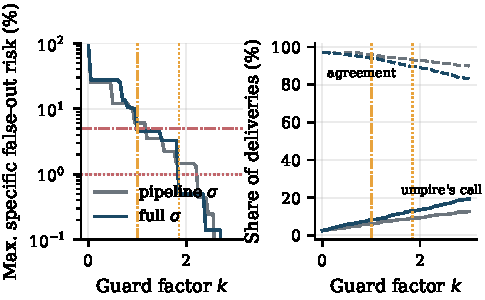
\includegraphics[width=\columnwidth]{risk.pdf}
\caption{Choice of the guard factor $\kappa$ on \RiskN{} simulated World~B deliveries with the calibrated
uncertainty. Left: largest JCGM~106 specific false-out risk among out calls against $\kappa$, with the 1 and
5\% limits. Right: verdict agreement (dashed) and share returned as umpire's call (solid). Vertical
lines: the chosen $\kappa$.}
\label{fig:risk}
\end{figure}

\end{document}
